\chapter{Benchmarking QUBO solvers}\label{benchmark}
This chapter first introduces related benchmarking work for QUBO problems and solvers. Then, we present the results of our benchmarking experiment.

\section{Related Benchmarking Work}
One of the first benchmarking works for quantum annealing was conducted by Denchev et al. \yrcite{denchev2016computational}, who measured the performance of D-Wave quantum annealing using a carefully crafted problem named weak-strong cluster networks, which has tall and narrow energy barriers separating local minima. For such problems with $\sim 10^3$ variables, quantum annealing is expected to be $\sim 10^8$ times faster to return the optimal solution compared to simulated annealing running on a single processor core. \outcite{Vert2021} used the maximum cardinality matching problem, a problem that is specially designed to be difficult for simulated annealing, and found that the D-Wave quantum annealer performs poorly compared to simulated annealing. Huang et al. \yrcite{Huang2023} conducted a recent benchmark study comparing the D-Wave quantum annealer, Fujitsu Digital Annealer and the GUROBI solver on the warehouse assignment problem. While the D-Wave annealer was the fastest solver, it yielded the worst solutions among all solvers tested.

For the QAOA solver, \outcite{b34} evaluated the performance of QAOA on the IBMQ backend and the D-Wave solver using instances of MaxCut and 2-satisfiability problems with up to 18 variables. The performance of the QAOA algorithm is inconsistent and underperforms quantum annealing in their problem set. \outcite{b32} compared simulated quantum annealing with QAOA with large values of $p$ and found that QAOA could find optimal solutions quicker than quantum annealing. However, the study only used small problems with sizes of $10-18$ and the parameter optimisation time for QAOA was omitted. More recently, \outcite{b35} also compared the performance of QAOA on the IBMQ backend and D-Wave quantum annealing on randomly generated Ising problems with cubic interaction terms and found that quantum annealing had superior performance over QAOA for all problem sizes. \outcite{Lykov2023} compared the QAOA solver with the GUROBI solver for max-cut problems on 3-regular graphs. They suggested that the QAOA solver would need to use $p > 11$ to match the performance of classical solvers for large graphs, which is greatly beyond what current quantum hardware can achieve.

\outcite{gomes2019classical} showed that the NNQS solving method with an RBM architecture produces high approximation ratio solutions for the max-cut problem with graph sizes of up to 256. \outcite{khandoker2023supplementing} uses recurrent neural networks as the NNQS architecture for the max-cut and travelling salesman problem and found that it outperforms simulated annealing. However, there has yet to be a direct study that compares quantum annealing, QAOA, and NNQS.

\section{Results and Discussion}
We present the performance metrics from the benchmarking experiment for each dataset, accompanied by error bars representing the unbiased standard error of the mean. Graphs with problem sizes on the x-axis are plotted with a log scale.

\subsection{NAE3SAT}
Performance by size for the NAE3SAT dataset is shown in \autoref{all-nae3sat-size}, and average performance is shown in \autoref{all-nae3sat-average}. The D-Wave and NNQS solvers could solve problems up to $n=300$. However, multiple embedding requests were required for problems of size $300$ for the D-Wave solver, which suggests that $n=300$ might be near the D-Wave solver's size limit for the NAE3SAT problem. The QAOA solver is limited to problems of up to $n=30$.

\begin{figure}[!htb]
    \centering
    \subfloat[Normalized energy]{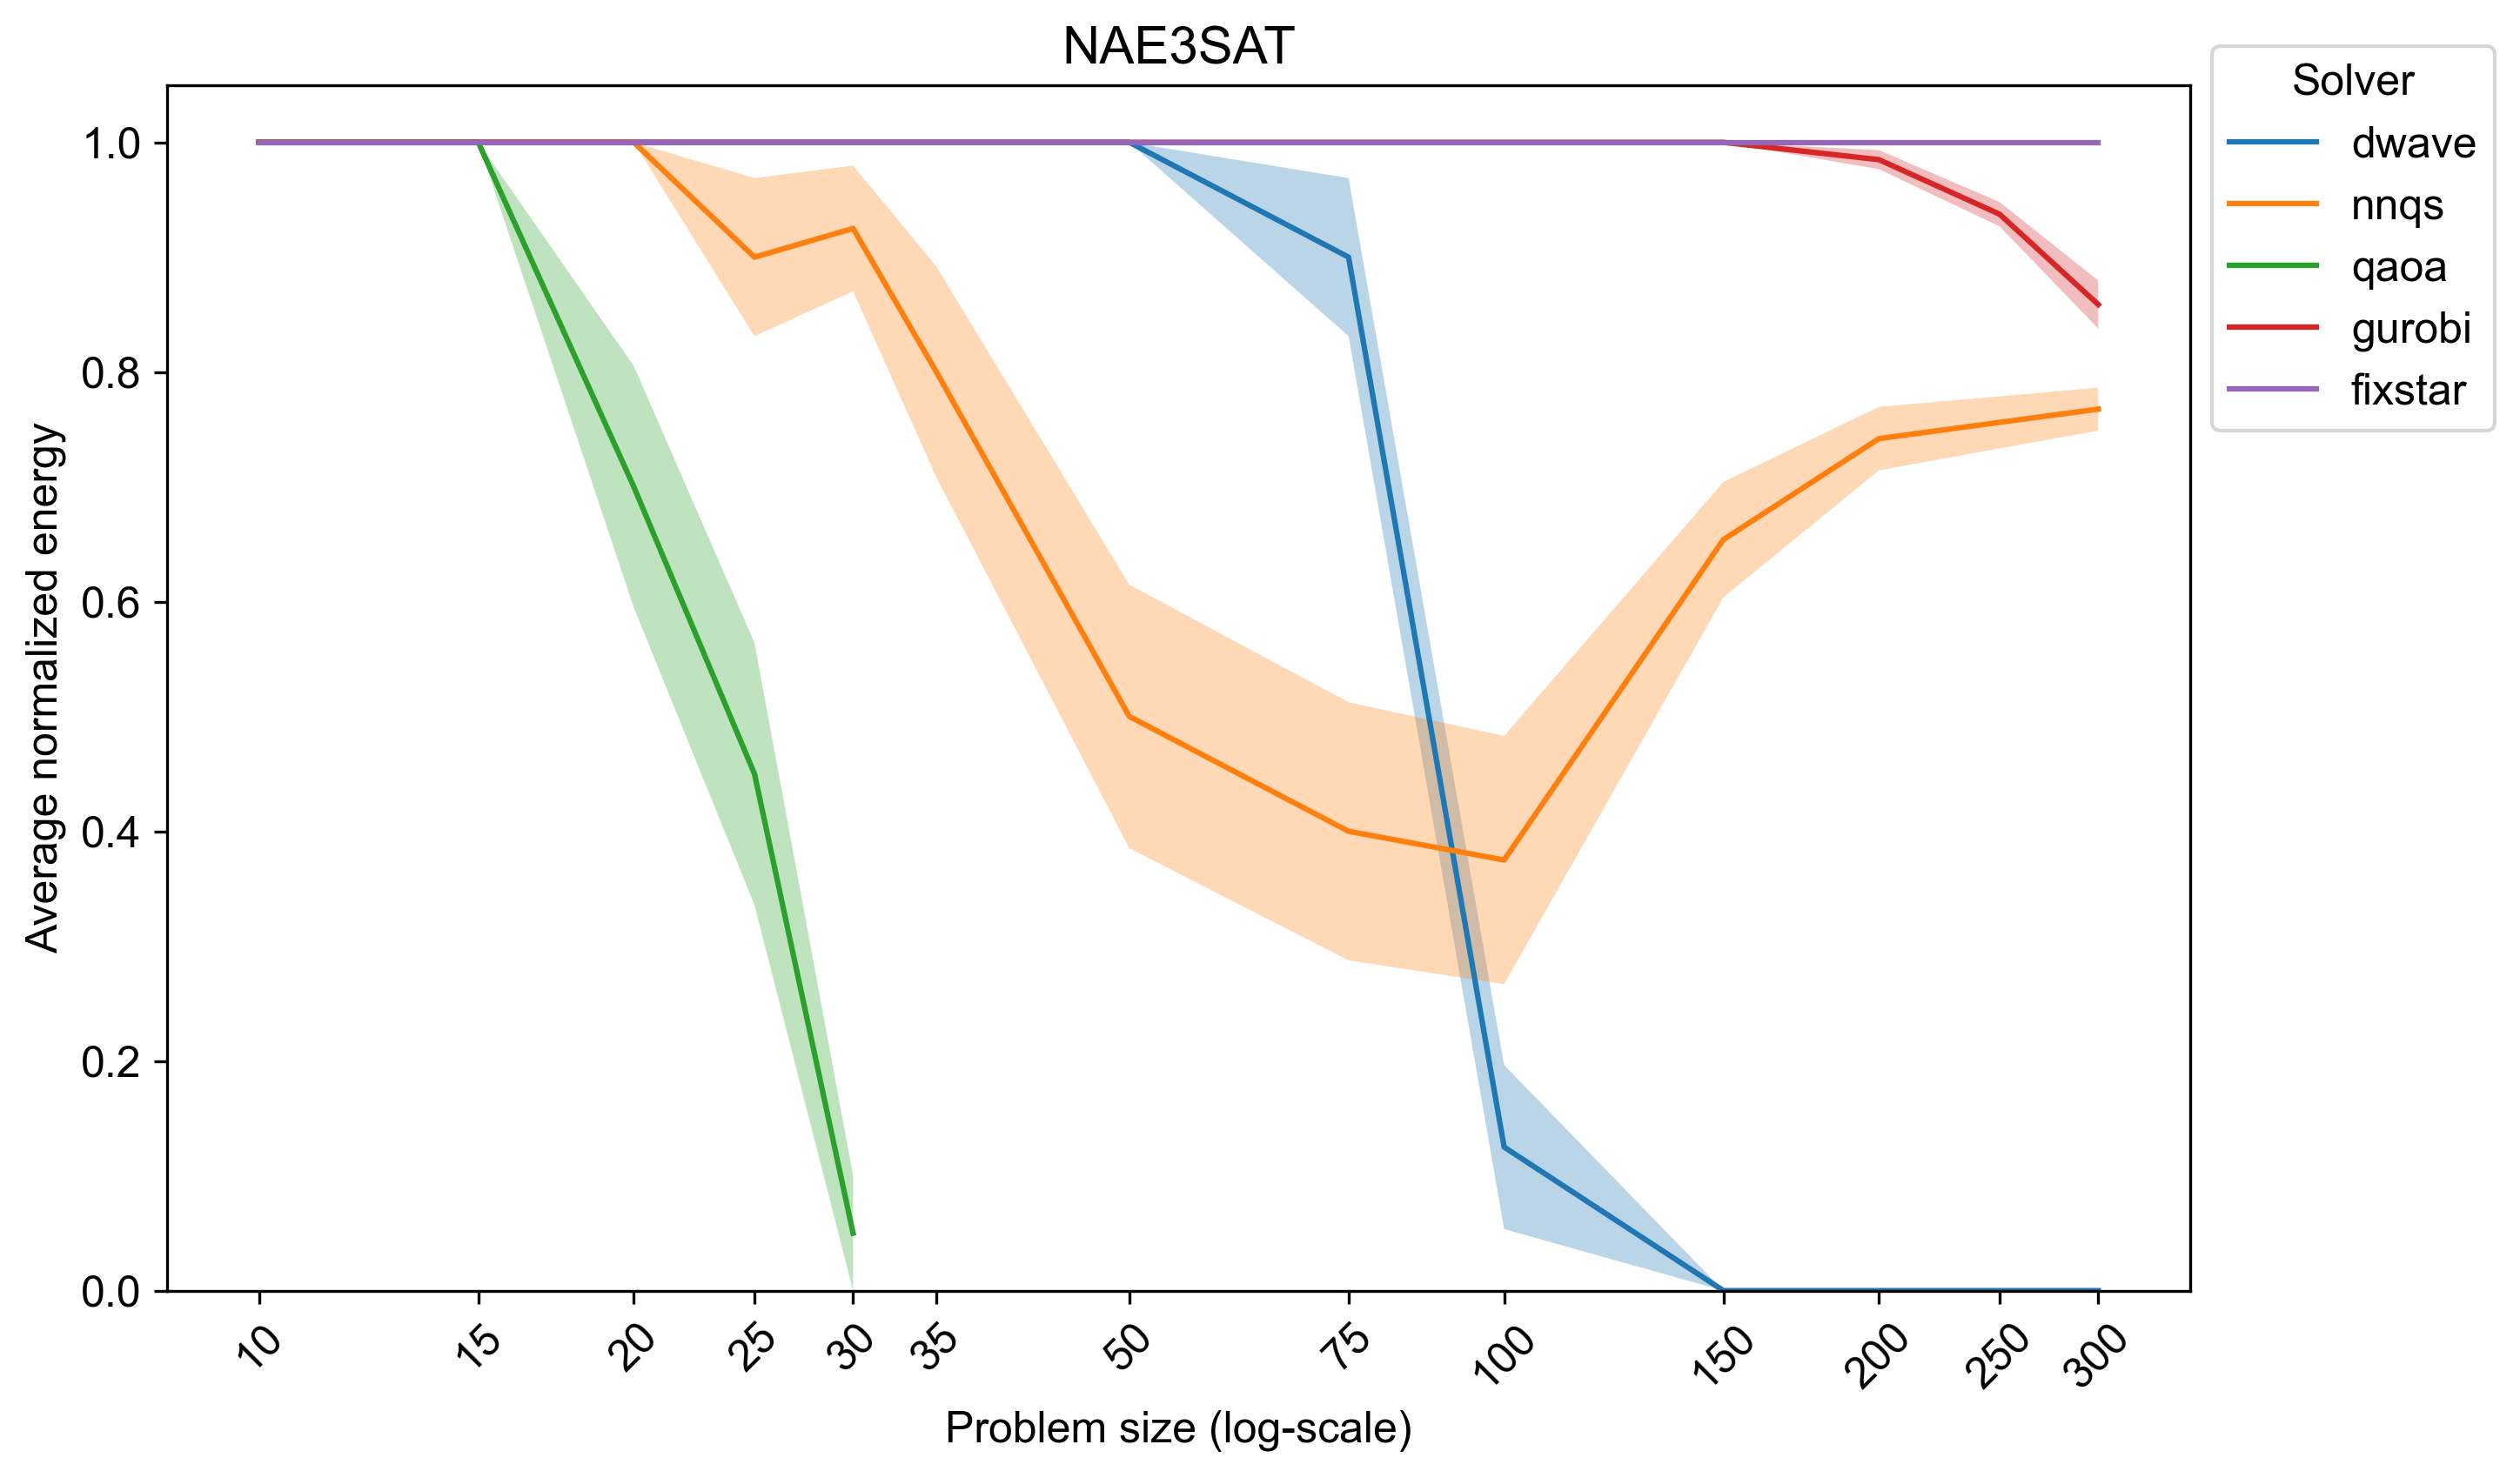
\includegraphics[width=0.5\textwidth]{images/nae3sat_all_size.png}}
    \subfloat[Success probability]{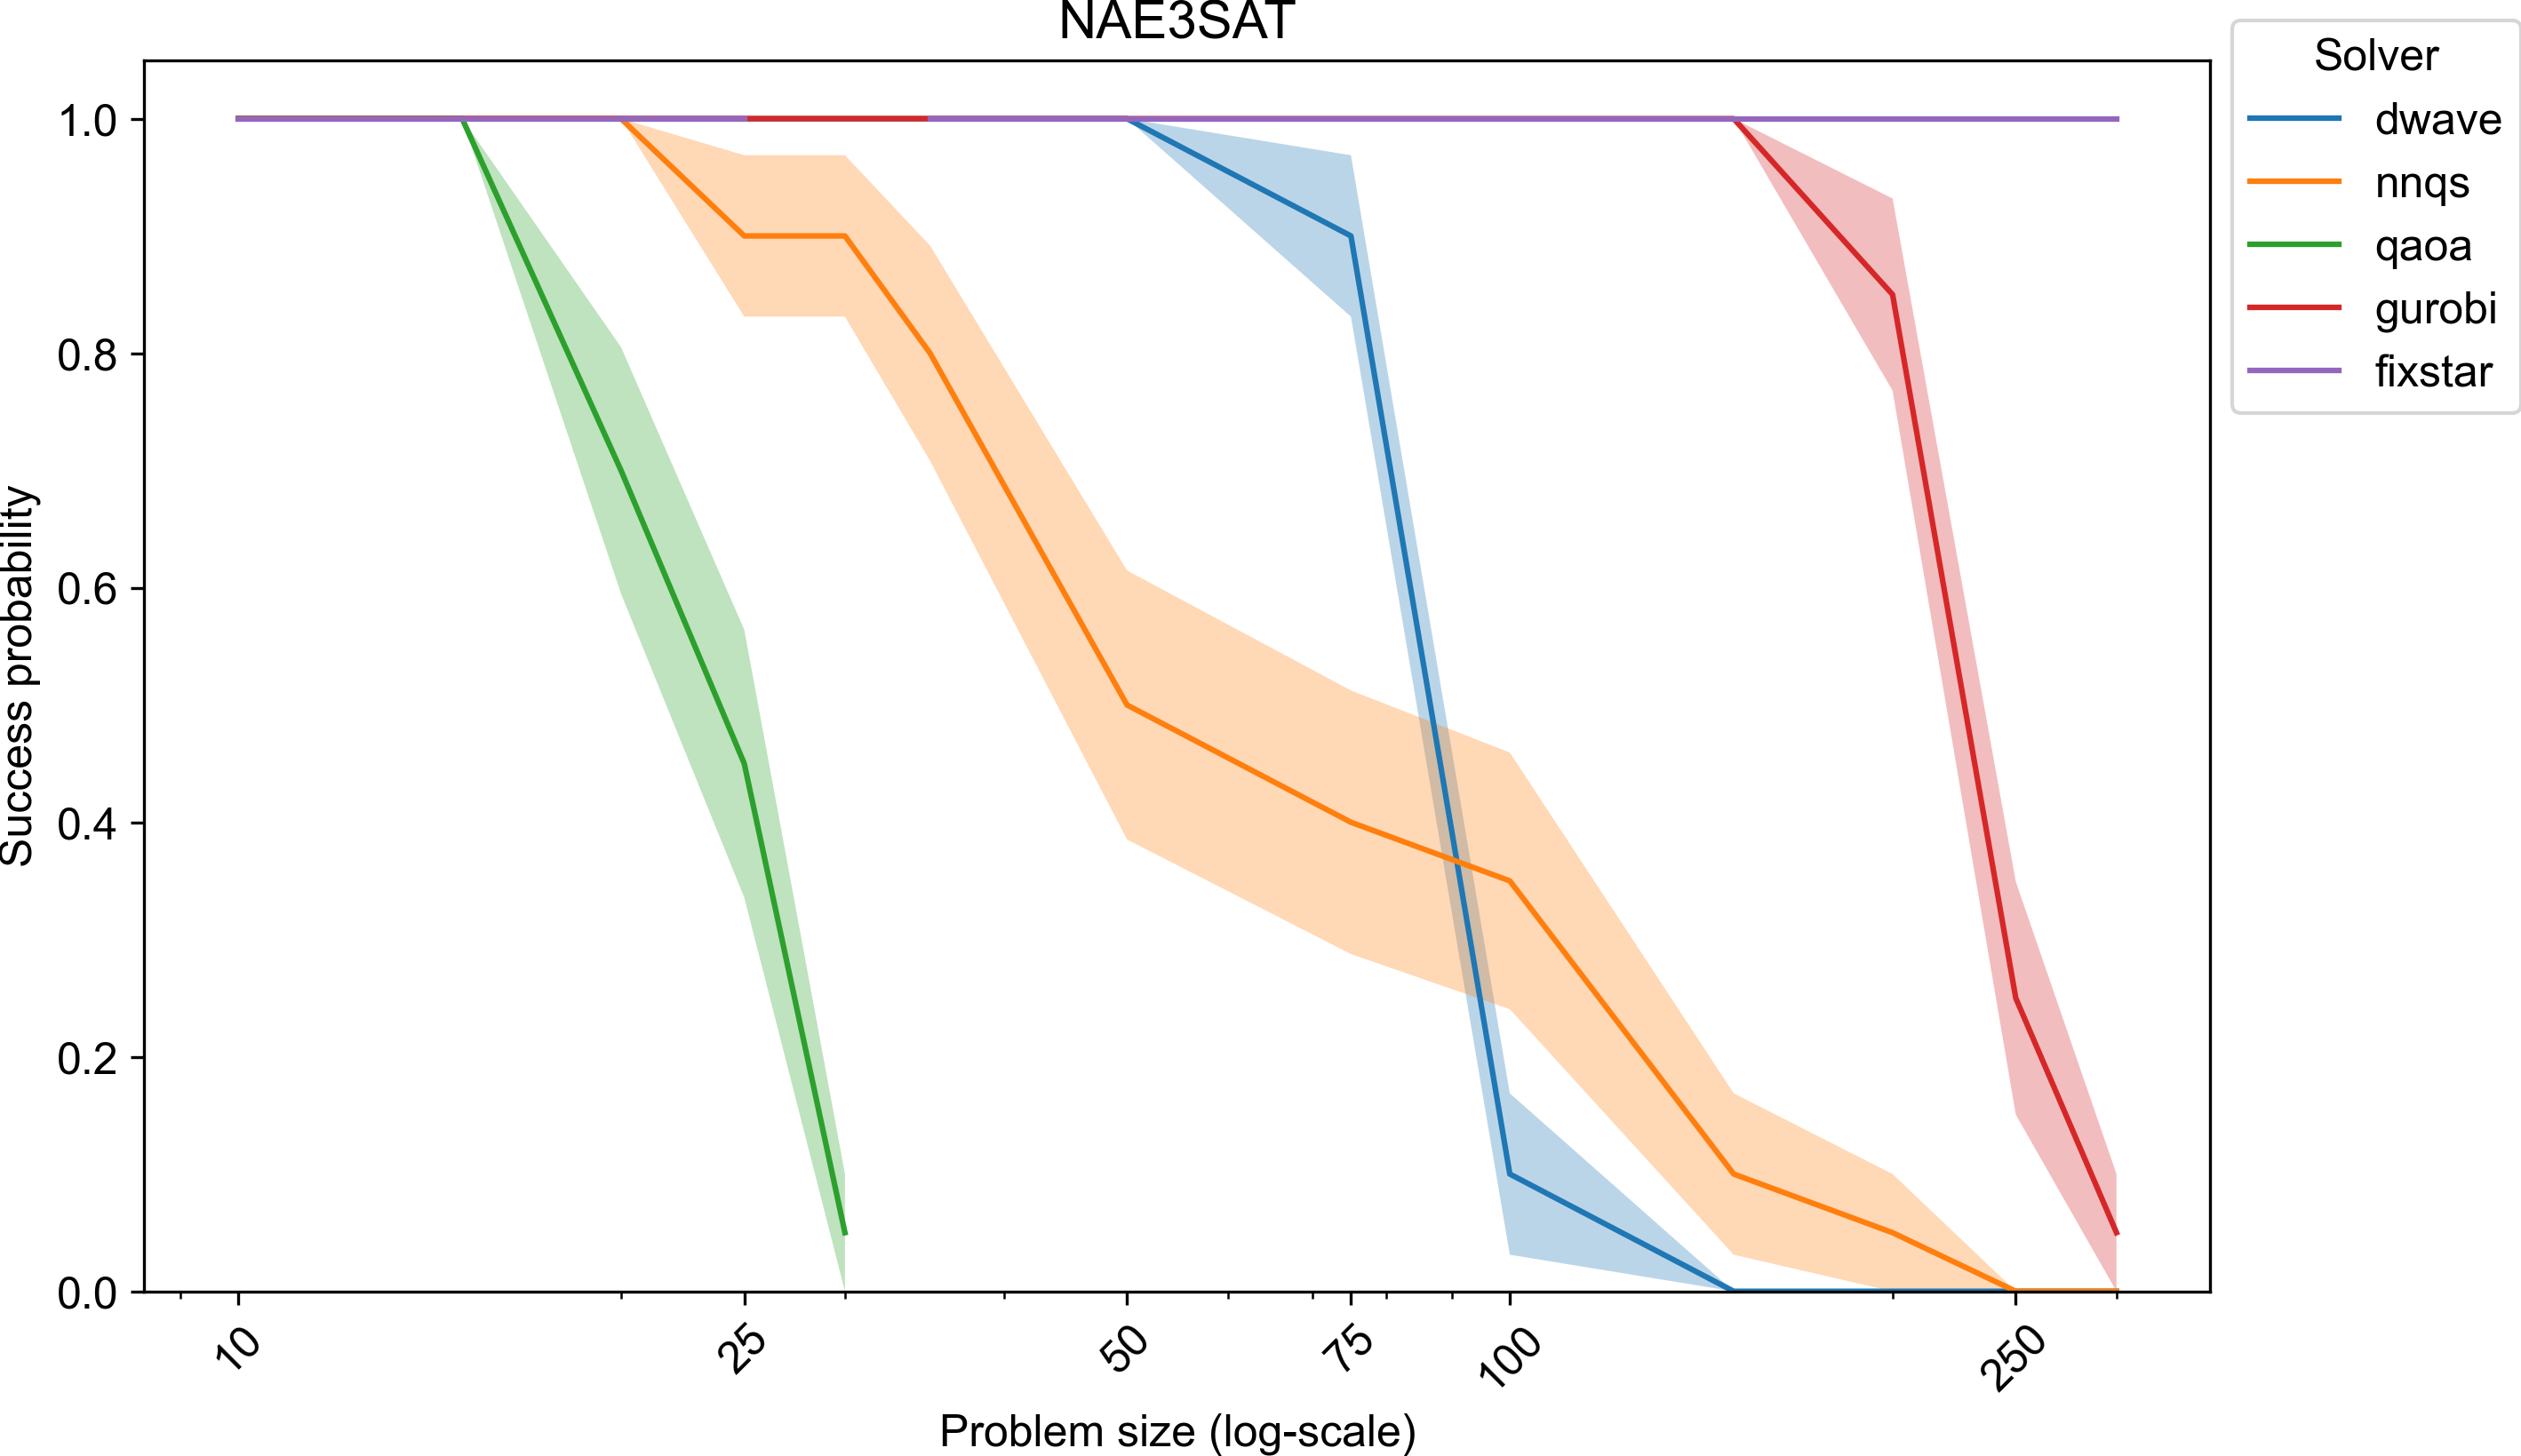
\includegraphics[width=0.5\textwidth]{images/nae3sat_all_success_size.png}}
    \caption{Performance of different solvers for NAE3SAT by problem size}
    \label{all-nae3sat-size}
\end{figure}

\begin{figure}[!htb]
    \centering
    \subfloat[Normalized energy]{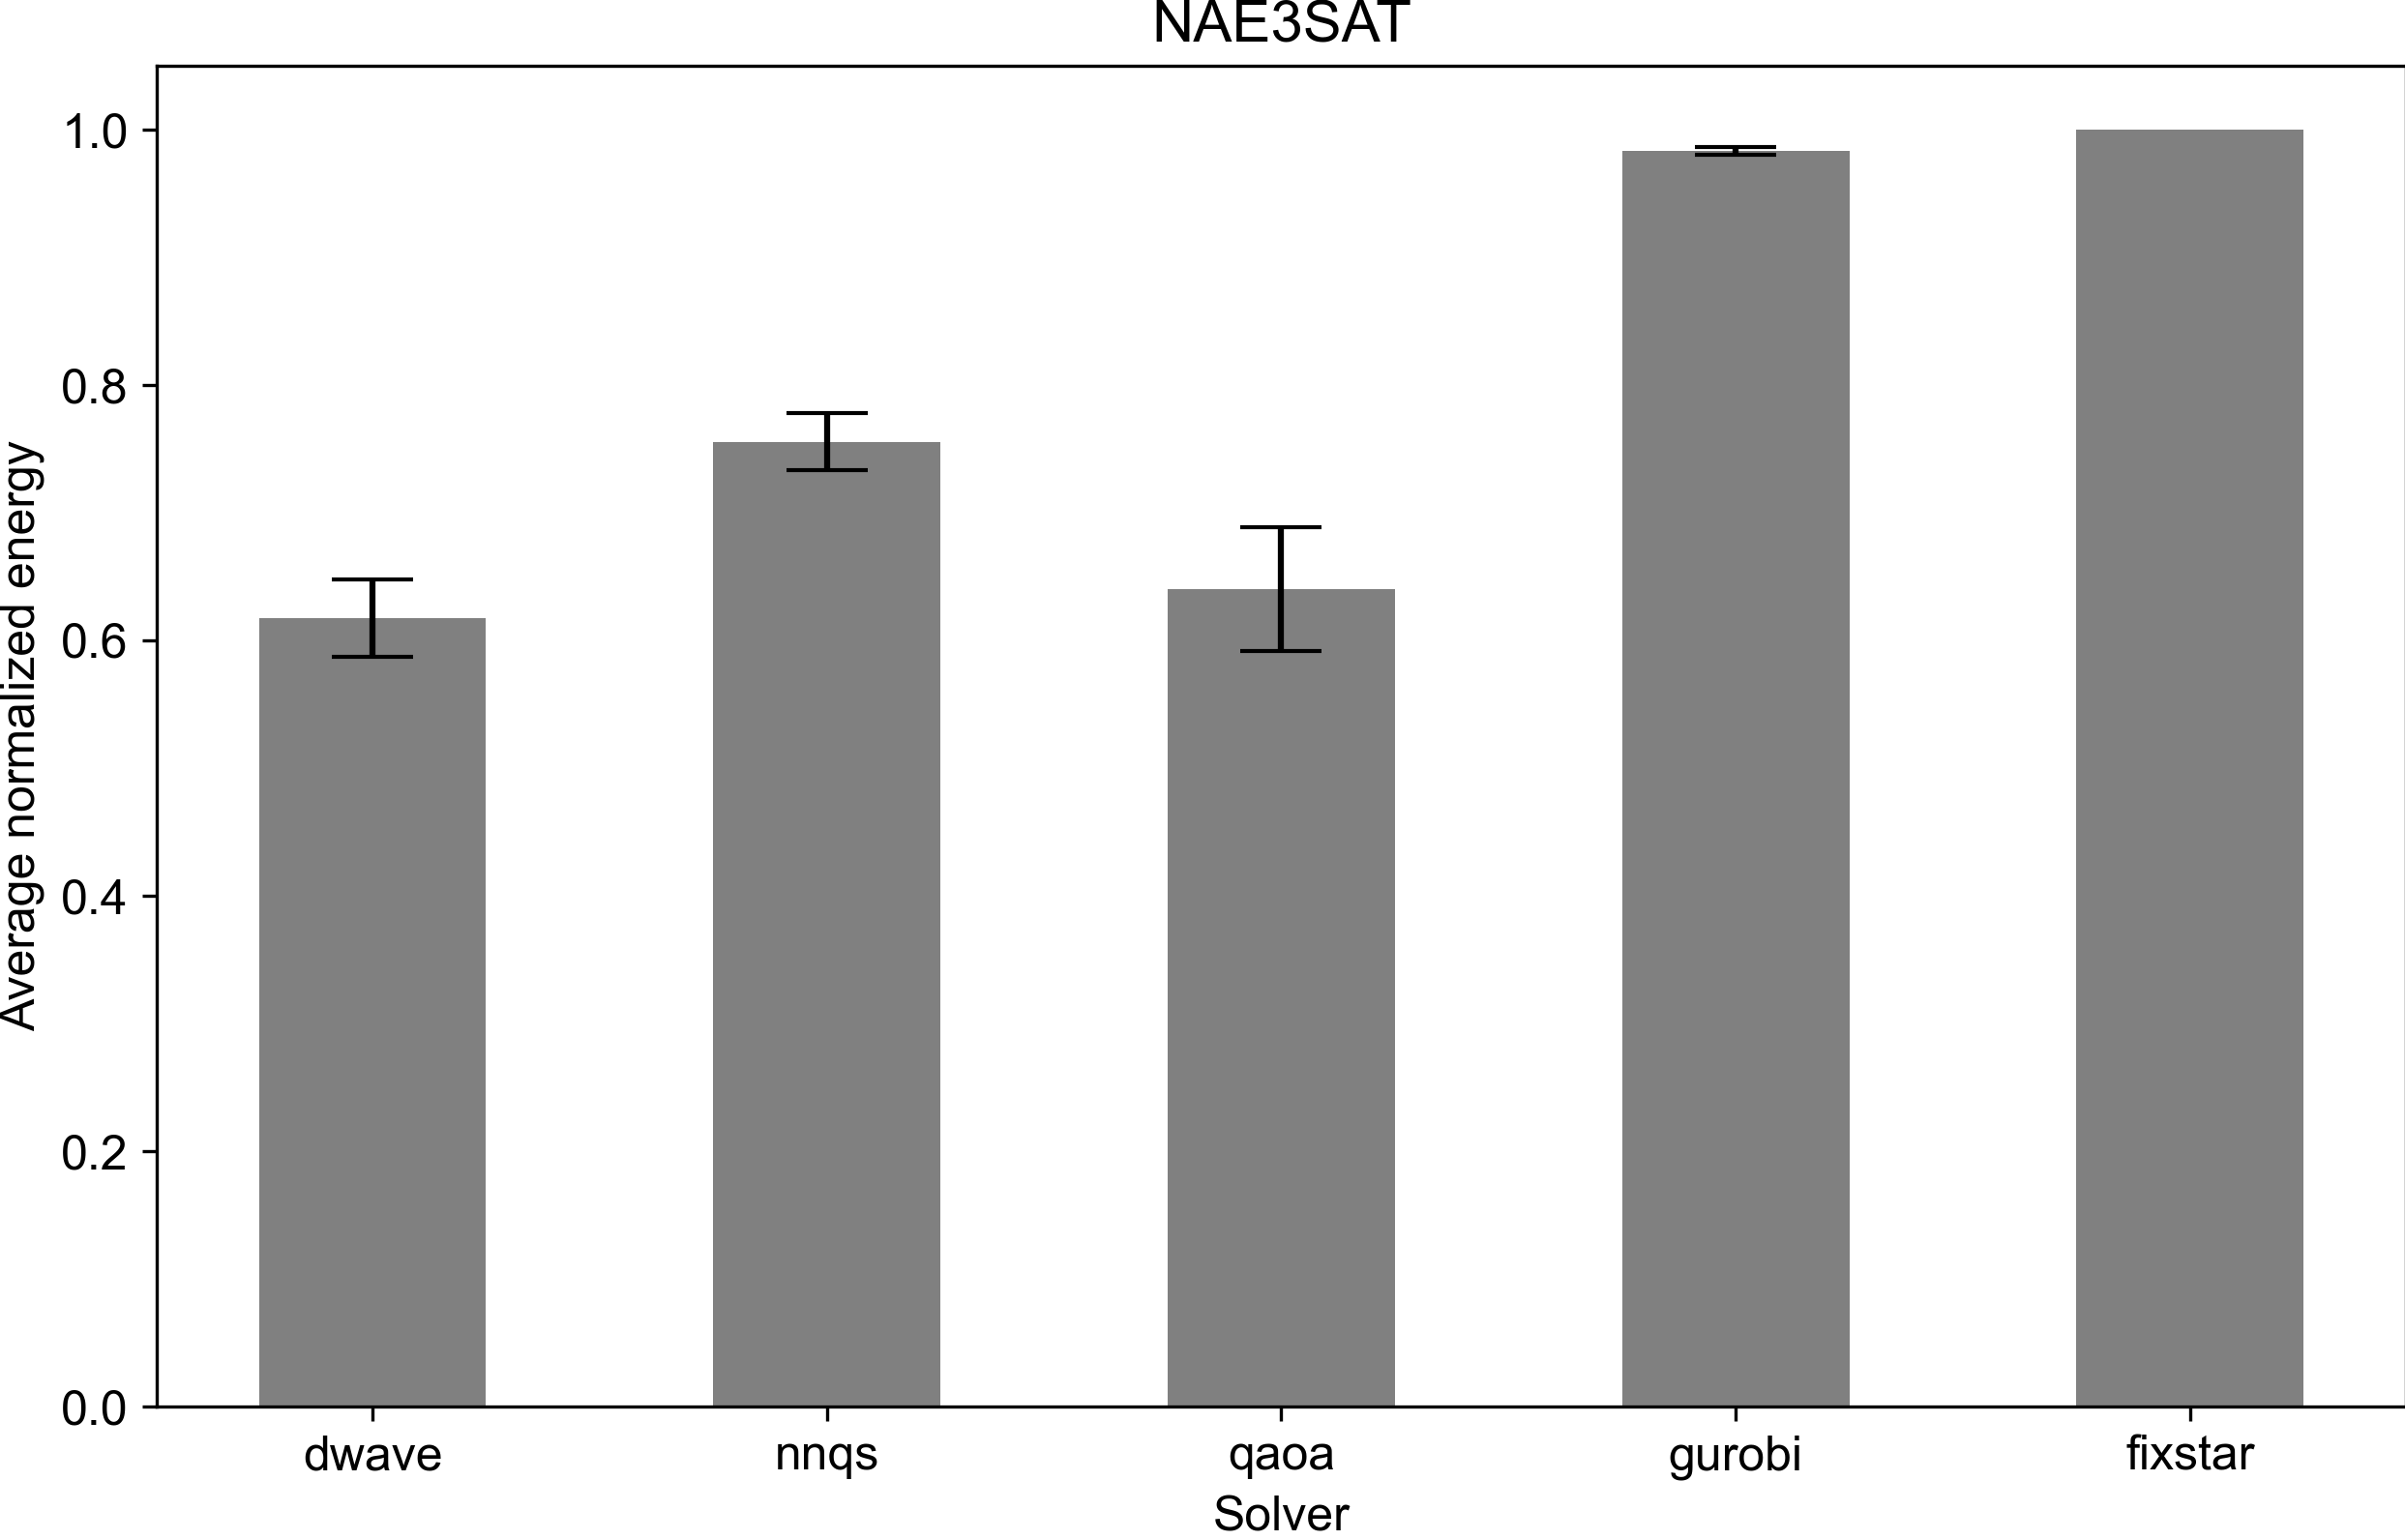
\includegraphics[width=0.4\textwidth]{images/nae3sat_all_avg.png}}\hspace{30px}
    \subfloat[Success probability]{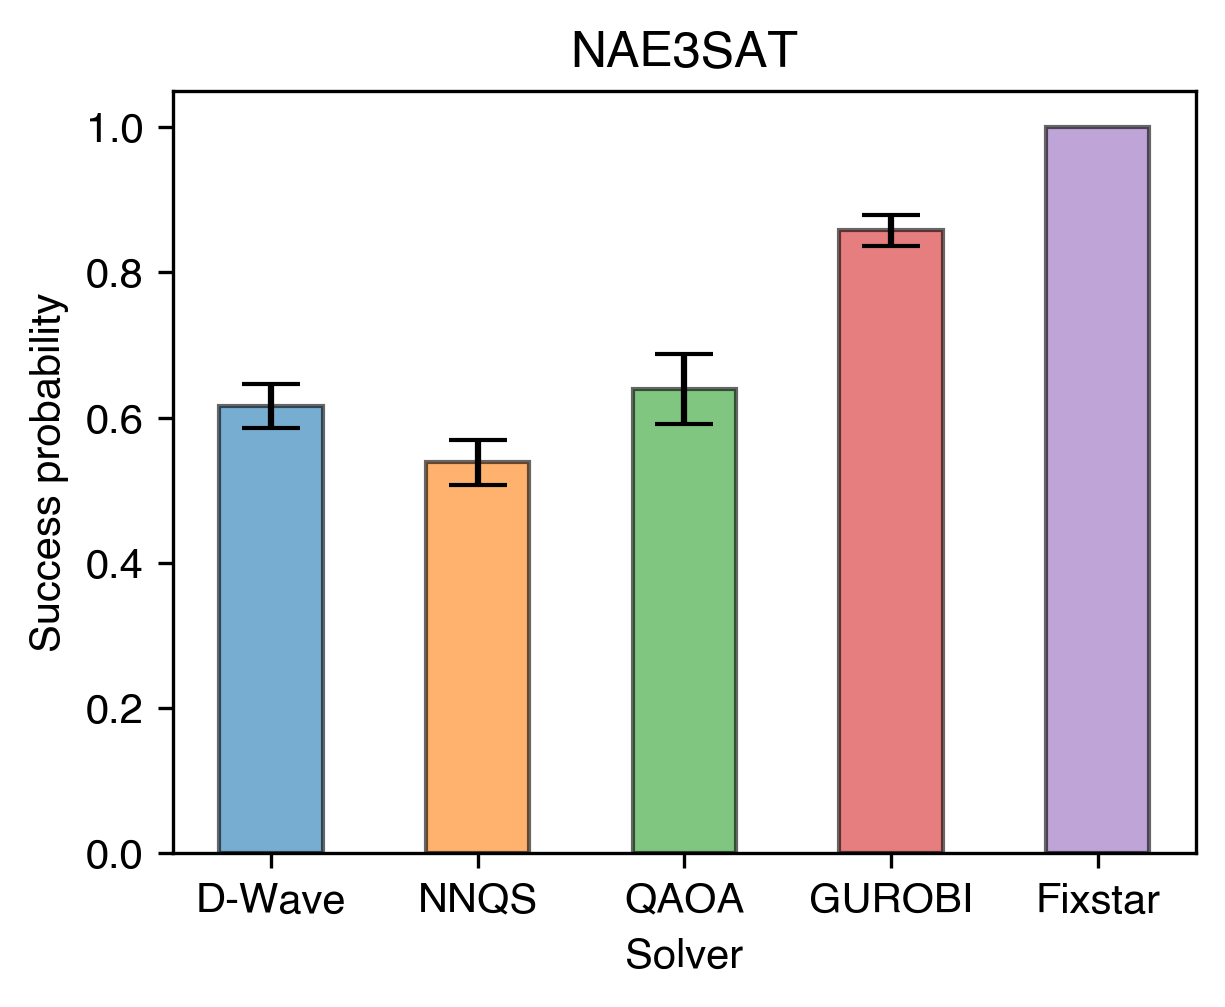
\includegraphics[width=0.4\textwidth]{images/nae3sat_all_success_avg.png}}
    \caption{Average performance of different solvers for NAE3SAT}
    \label{all-nae3sat-average}
\end{figure}

The D-Wave solver performs well up to $n=50$ with a success probability of $1$. For larger problem sizes, the performance of the D-Wave solver drops off sharply. The NNQS solver performs well up to $n=20$, with the success probability and normalised energy gradually decreasing as the problem size increases until $n=300$. The QAOA solver performs well up to $n=15$, and performance decreases until $n=30$. Among the classical solvers, the Fixstar solver performs better than the GUROBI solver at larger problem sizes ($>150$). Both classical solvers outperform the quantum-inspired solvers.

Overall, the NNQS has the highest average normalised energy among the three quantum-inspired solvers but has the lowest success probability, which is likely due to it being able to solve problems of larger sizes that the D-Wave Annealer and QAOA solver cannot handle. The QAOA solver has the highest success probability but can only handle problems up to $n=30$. Both classical solvers outperform the quantum-inspired solvers.

\subsection{Max-cut}
Performance by size for the max-cut dataset is shown in \autoref{all-maxcut-size}, and average performance is shown in \autoref{all-maxcut-average}. The D-Wave solver could only handle max-cut problems of sizes up to $n=150$ due to the need for minor embedding onto the QPU's pegasus topology. The max-cut problem requires $\sim 0.25n$ edges per vertex, making the embedding challenging for large $n$. The NNQS solver could solve problems up to $n=300$. The QAOA solver is limited to problems of up to $n=30$.

\begin{figure}[!htb]
    \centering
    \subfloat[Normalized energy]{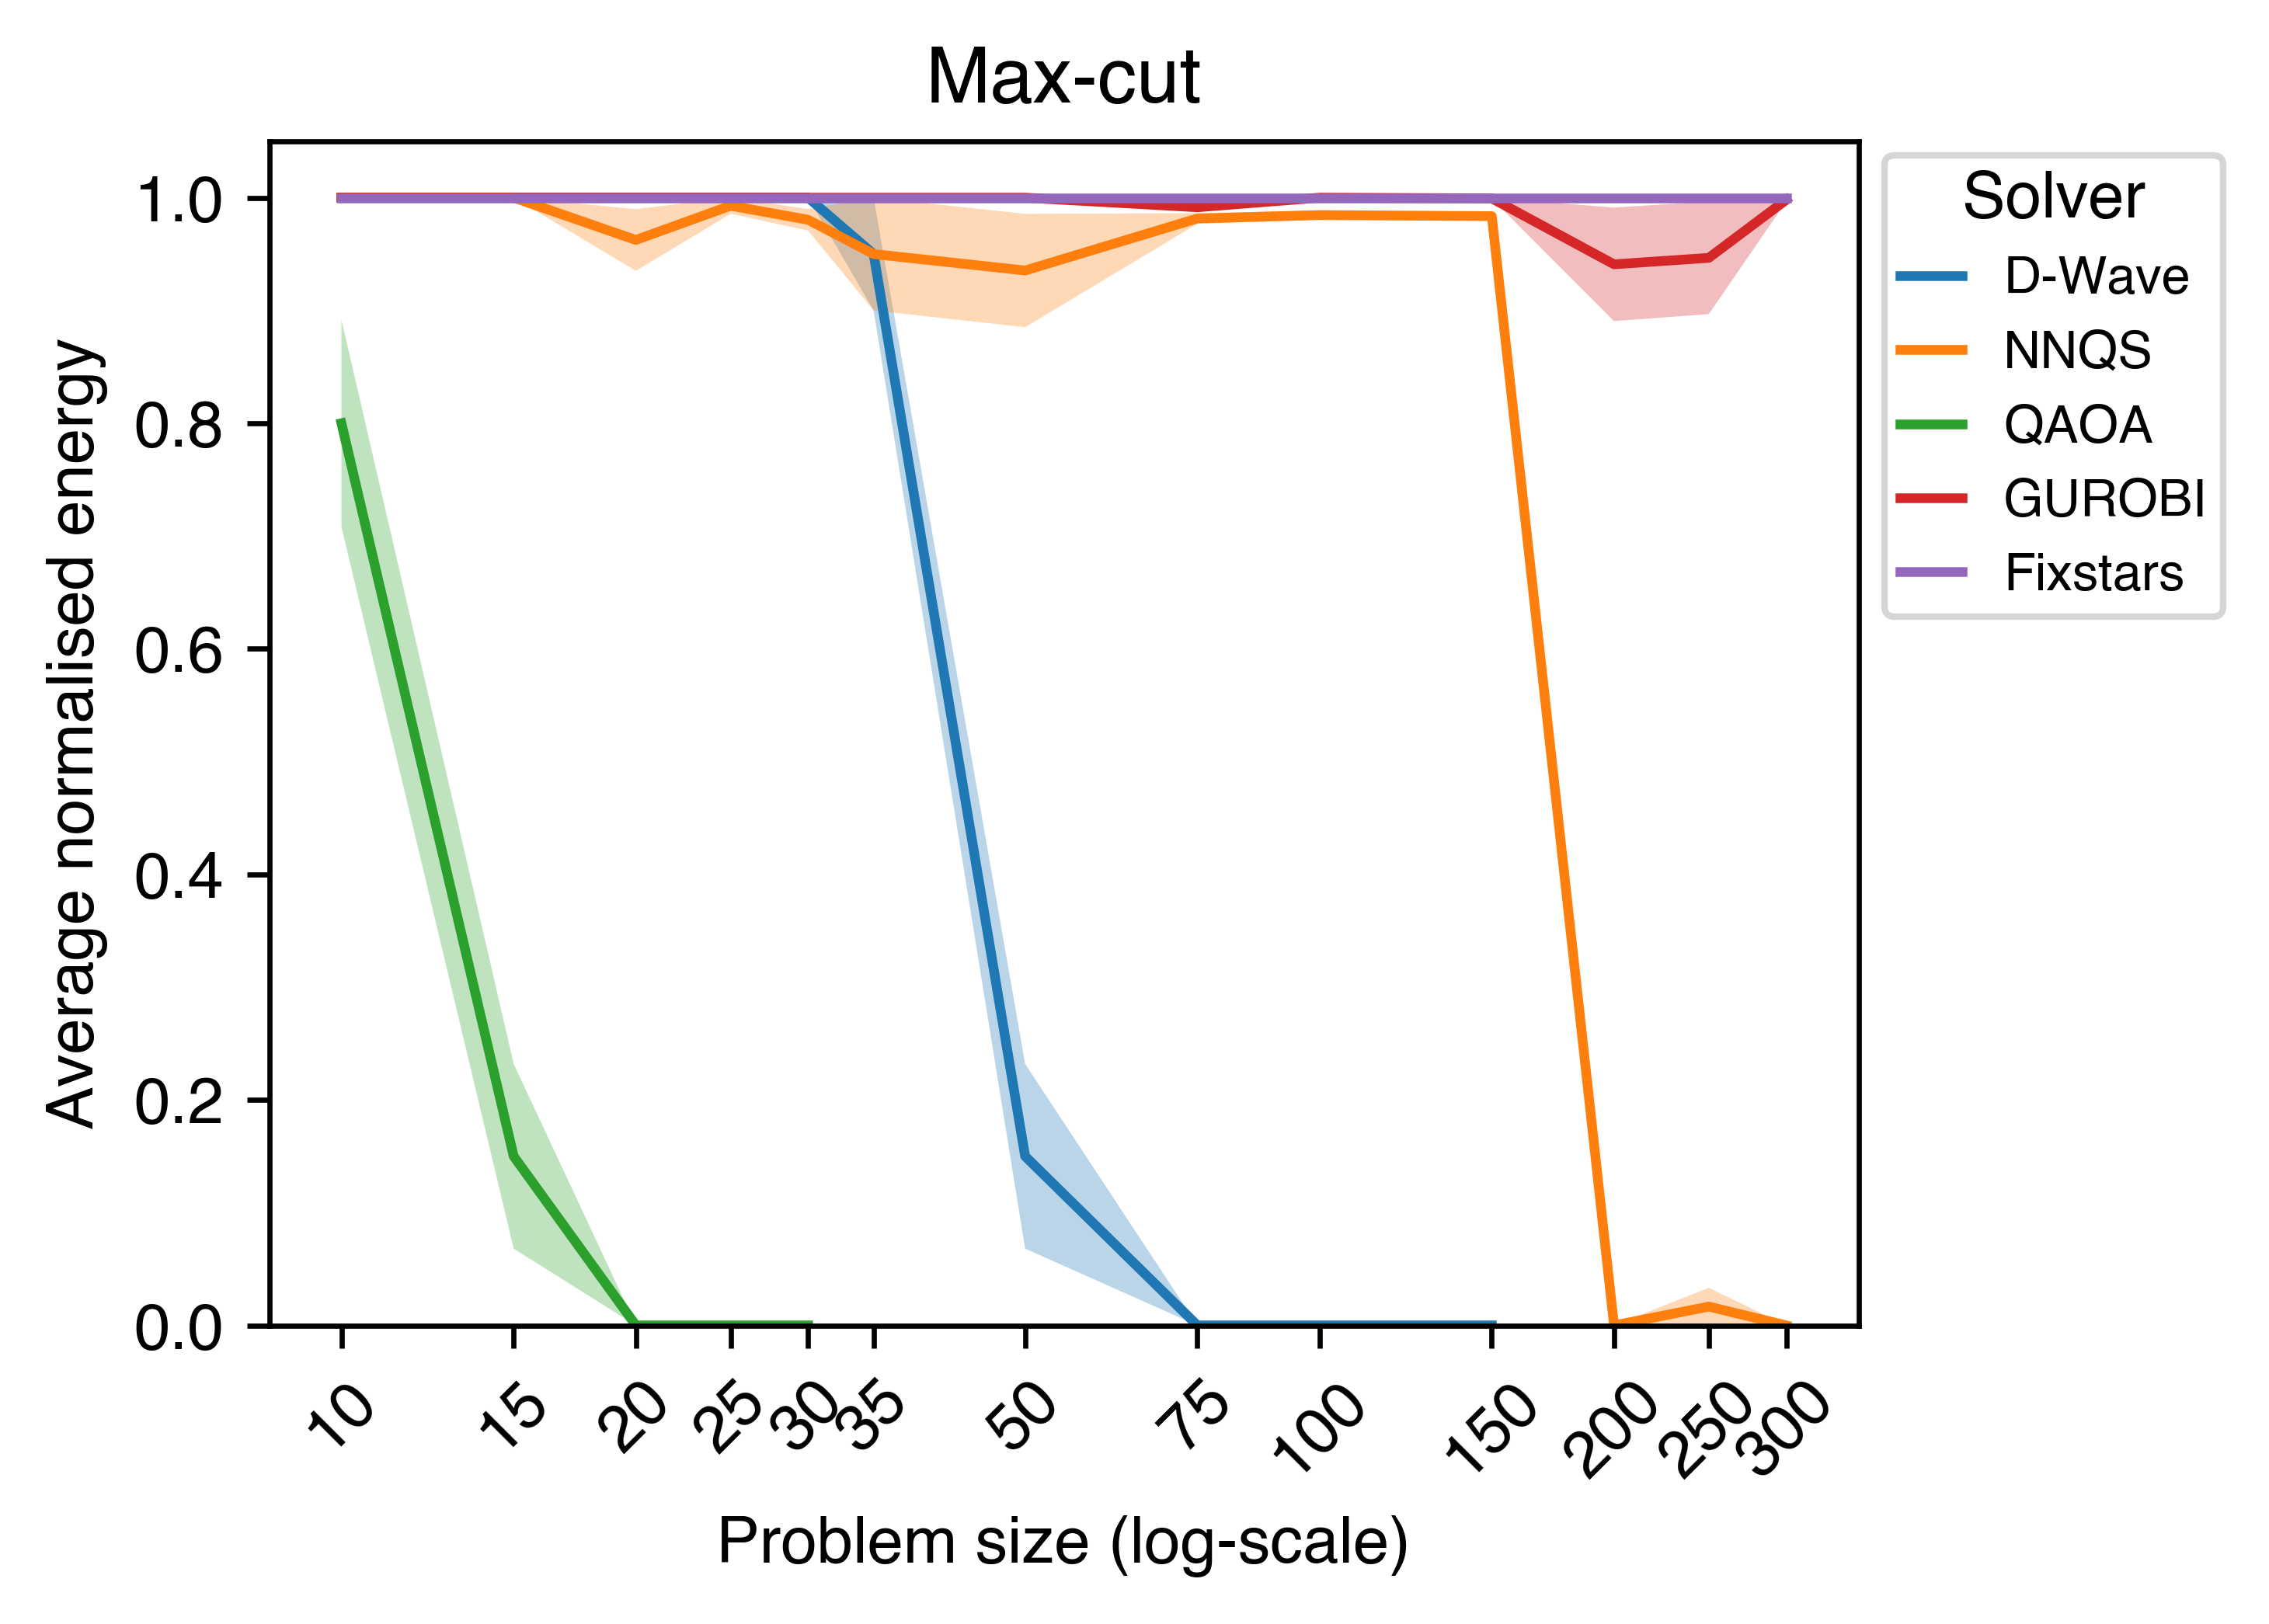
\includegraphics[width=0.5\textwidth]{images/maxcut_all_size.png}}
    \subfloat[Success probability]{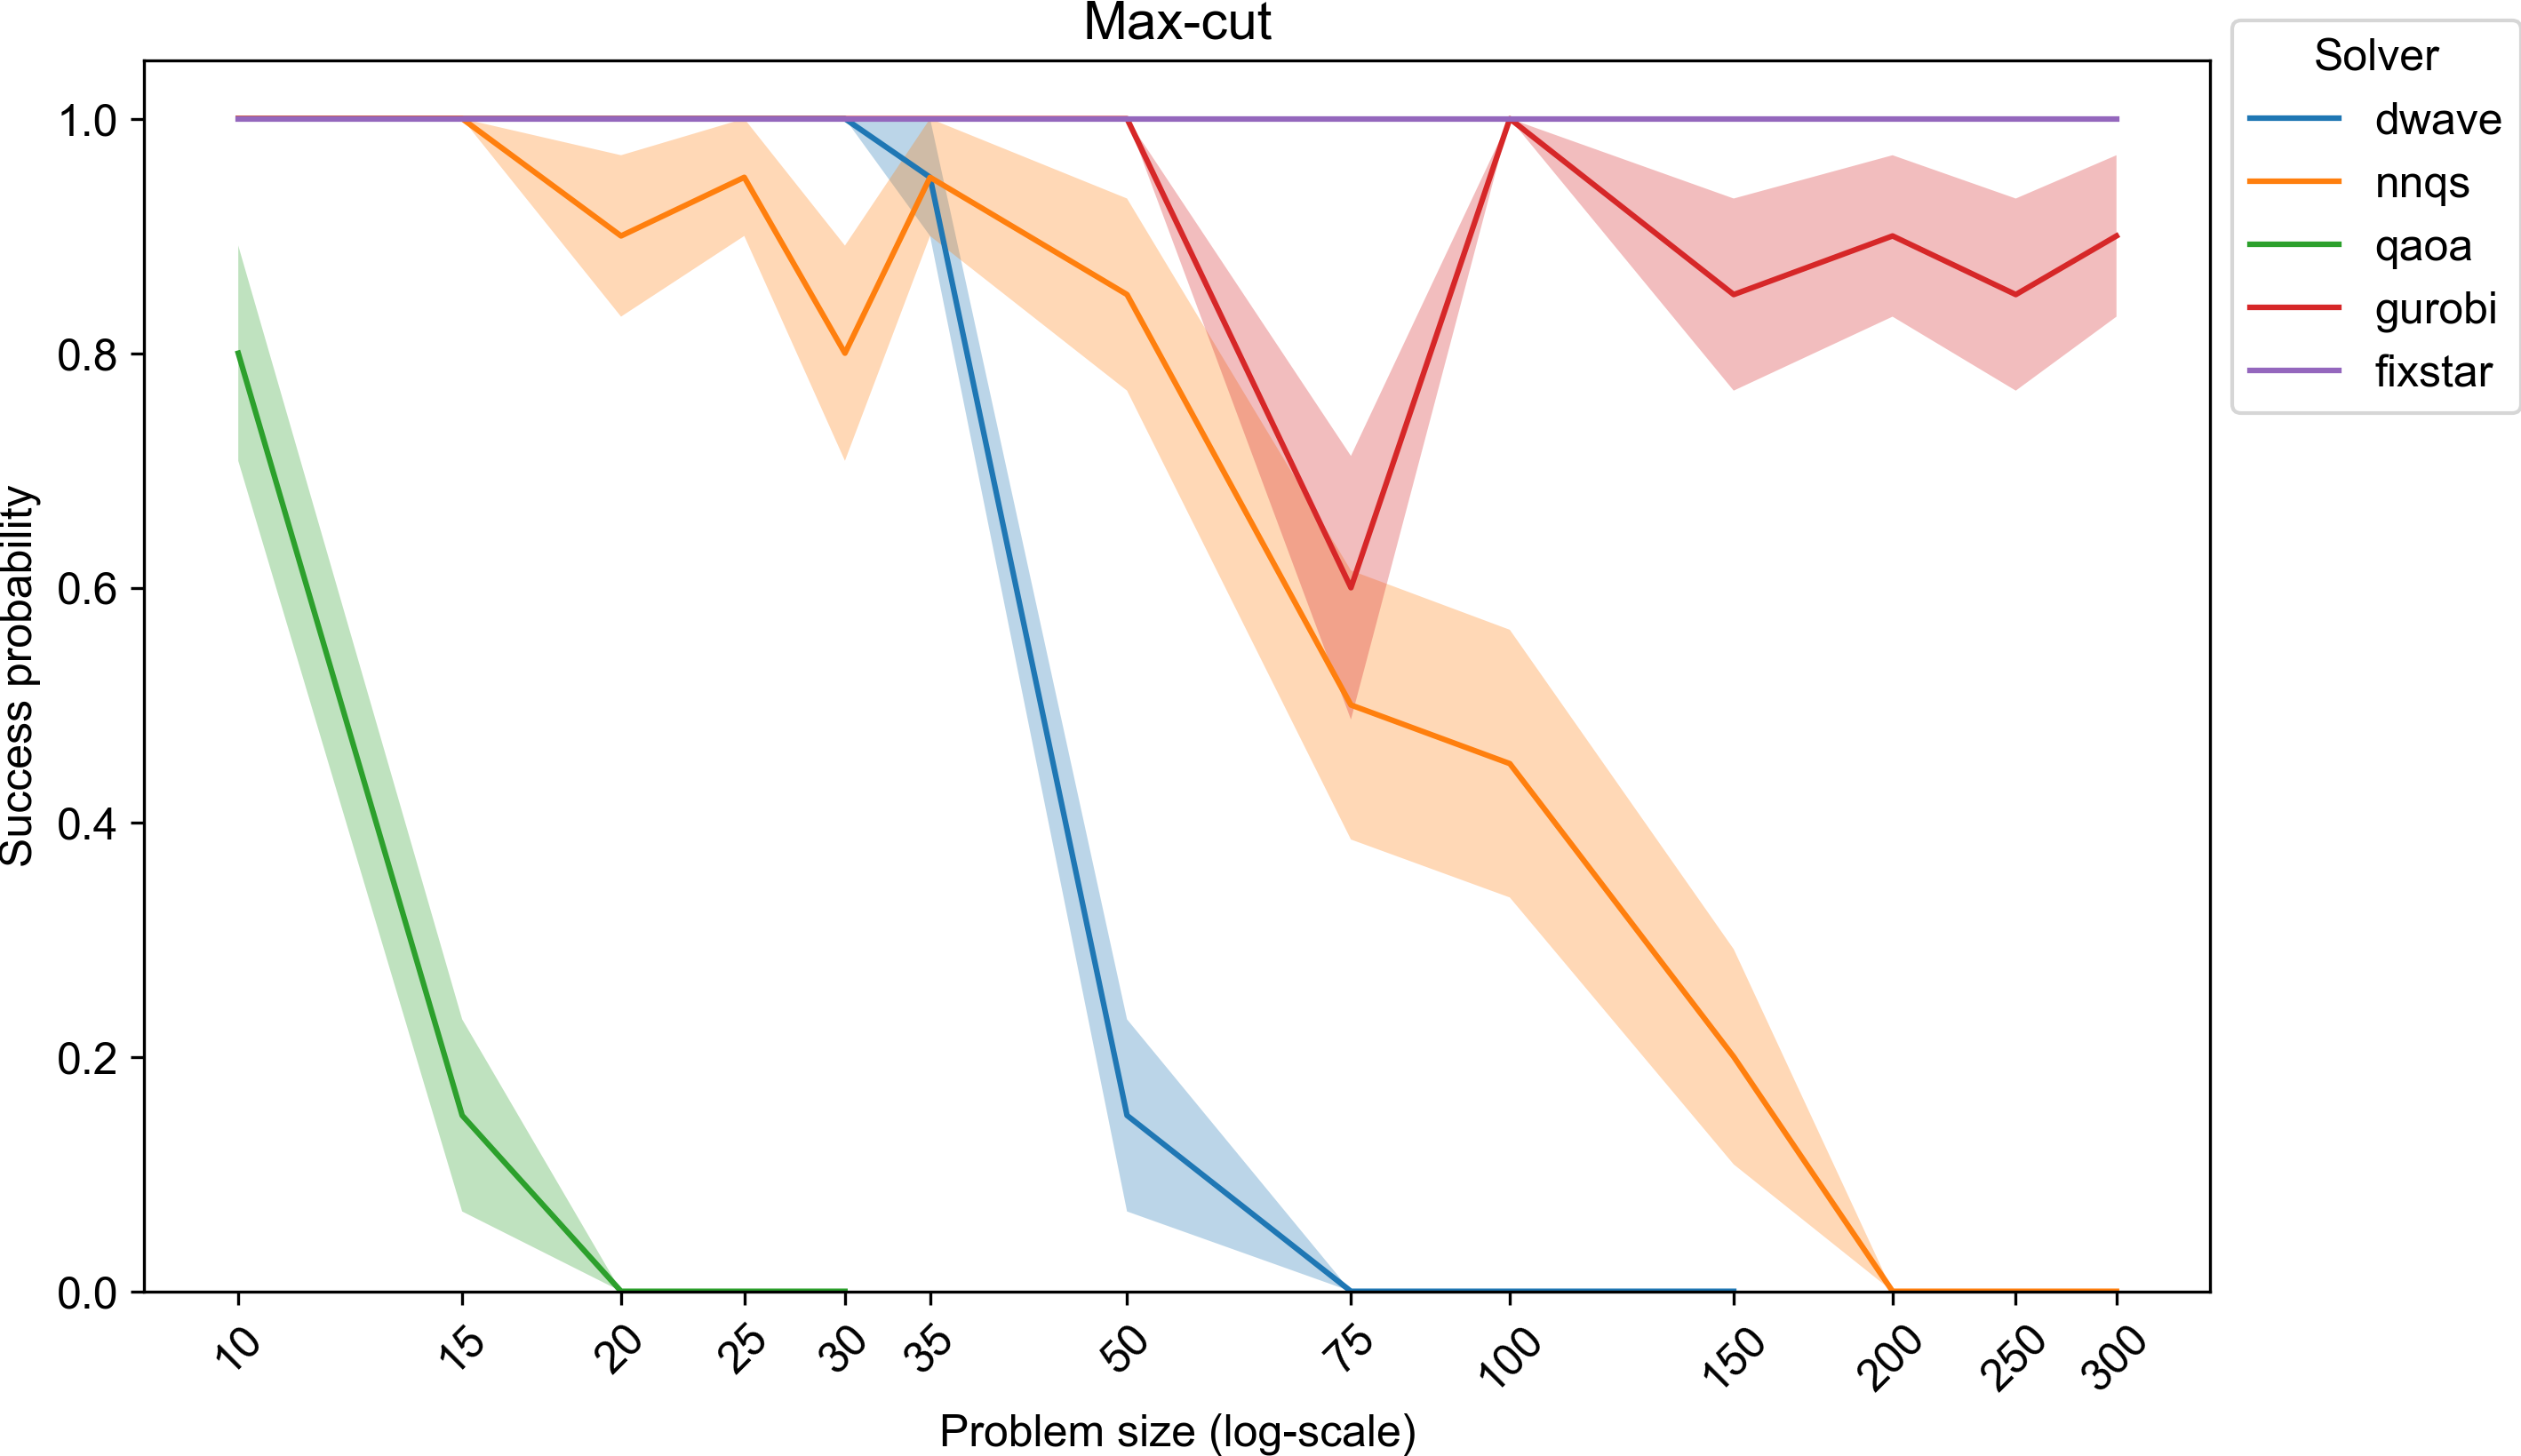
\includegraphics[width=0.5\textwidth]{images/maxcut_all_success_size.png}}
    \caption{Performance of different solvers for max-cut by problem size}
    \label{all-maxcut-size}
\end{figure}

\begin{figure}[!htb]
    \centering
    \subfloat[Normalized energy]{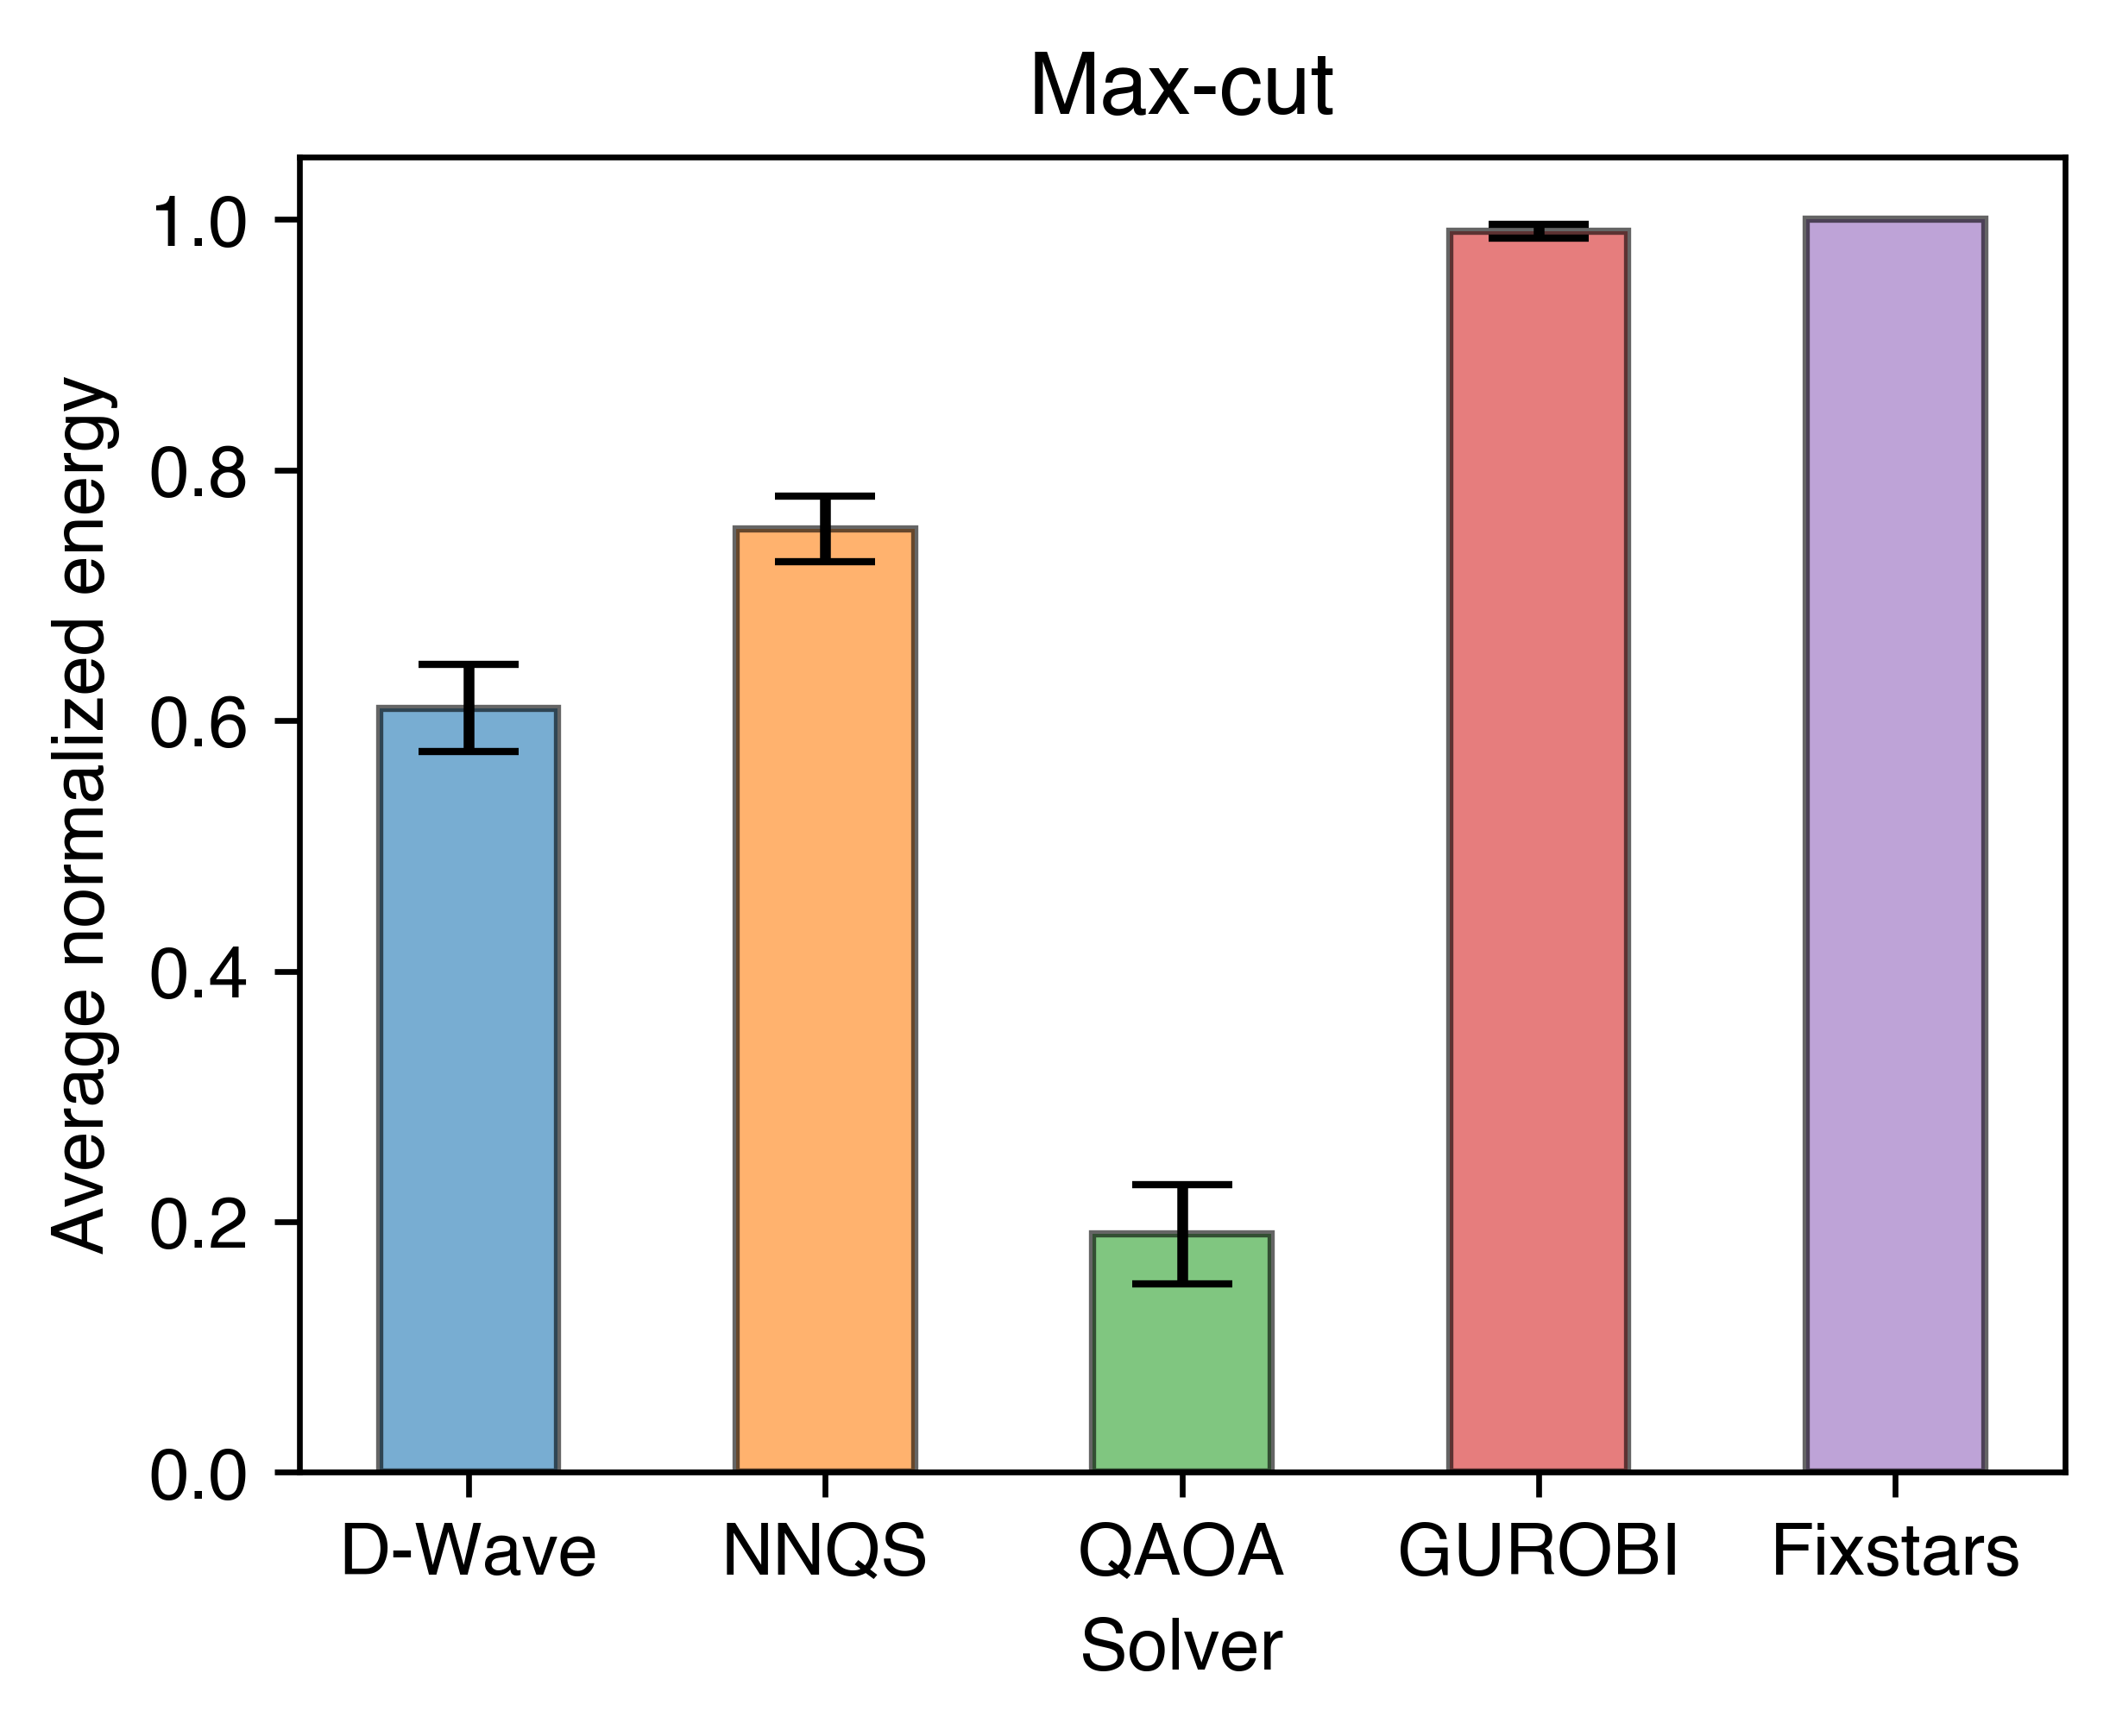
\includegraphics[width=0.4\textwidth]{images/maxcut_all_avg.png}}\hspace{30px}
    \subfloat[Success probability]{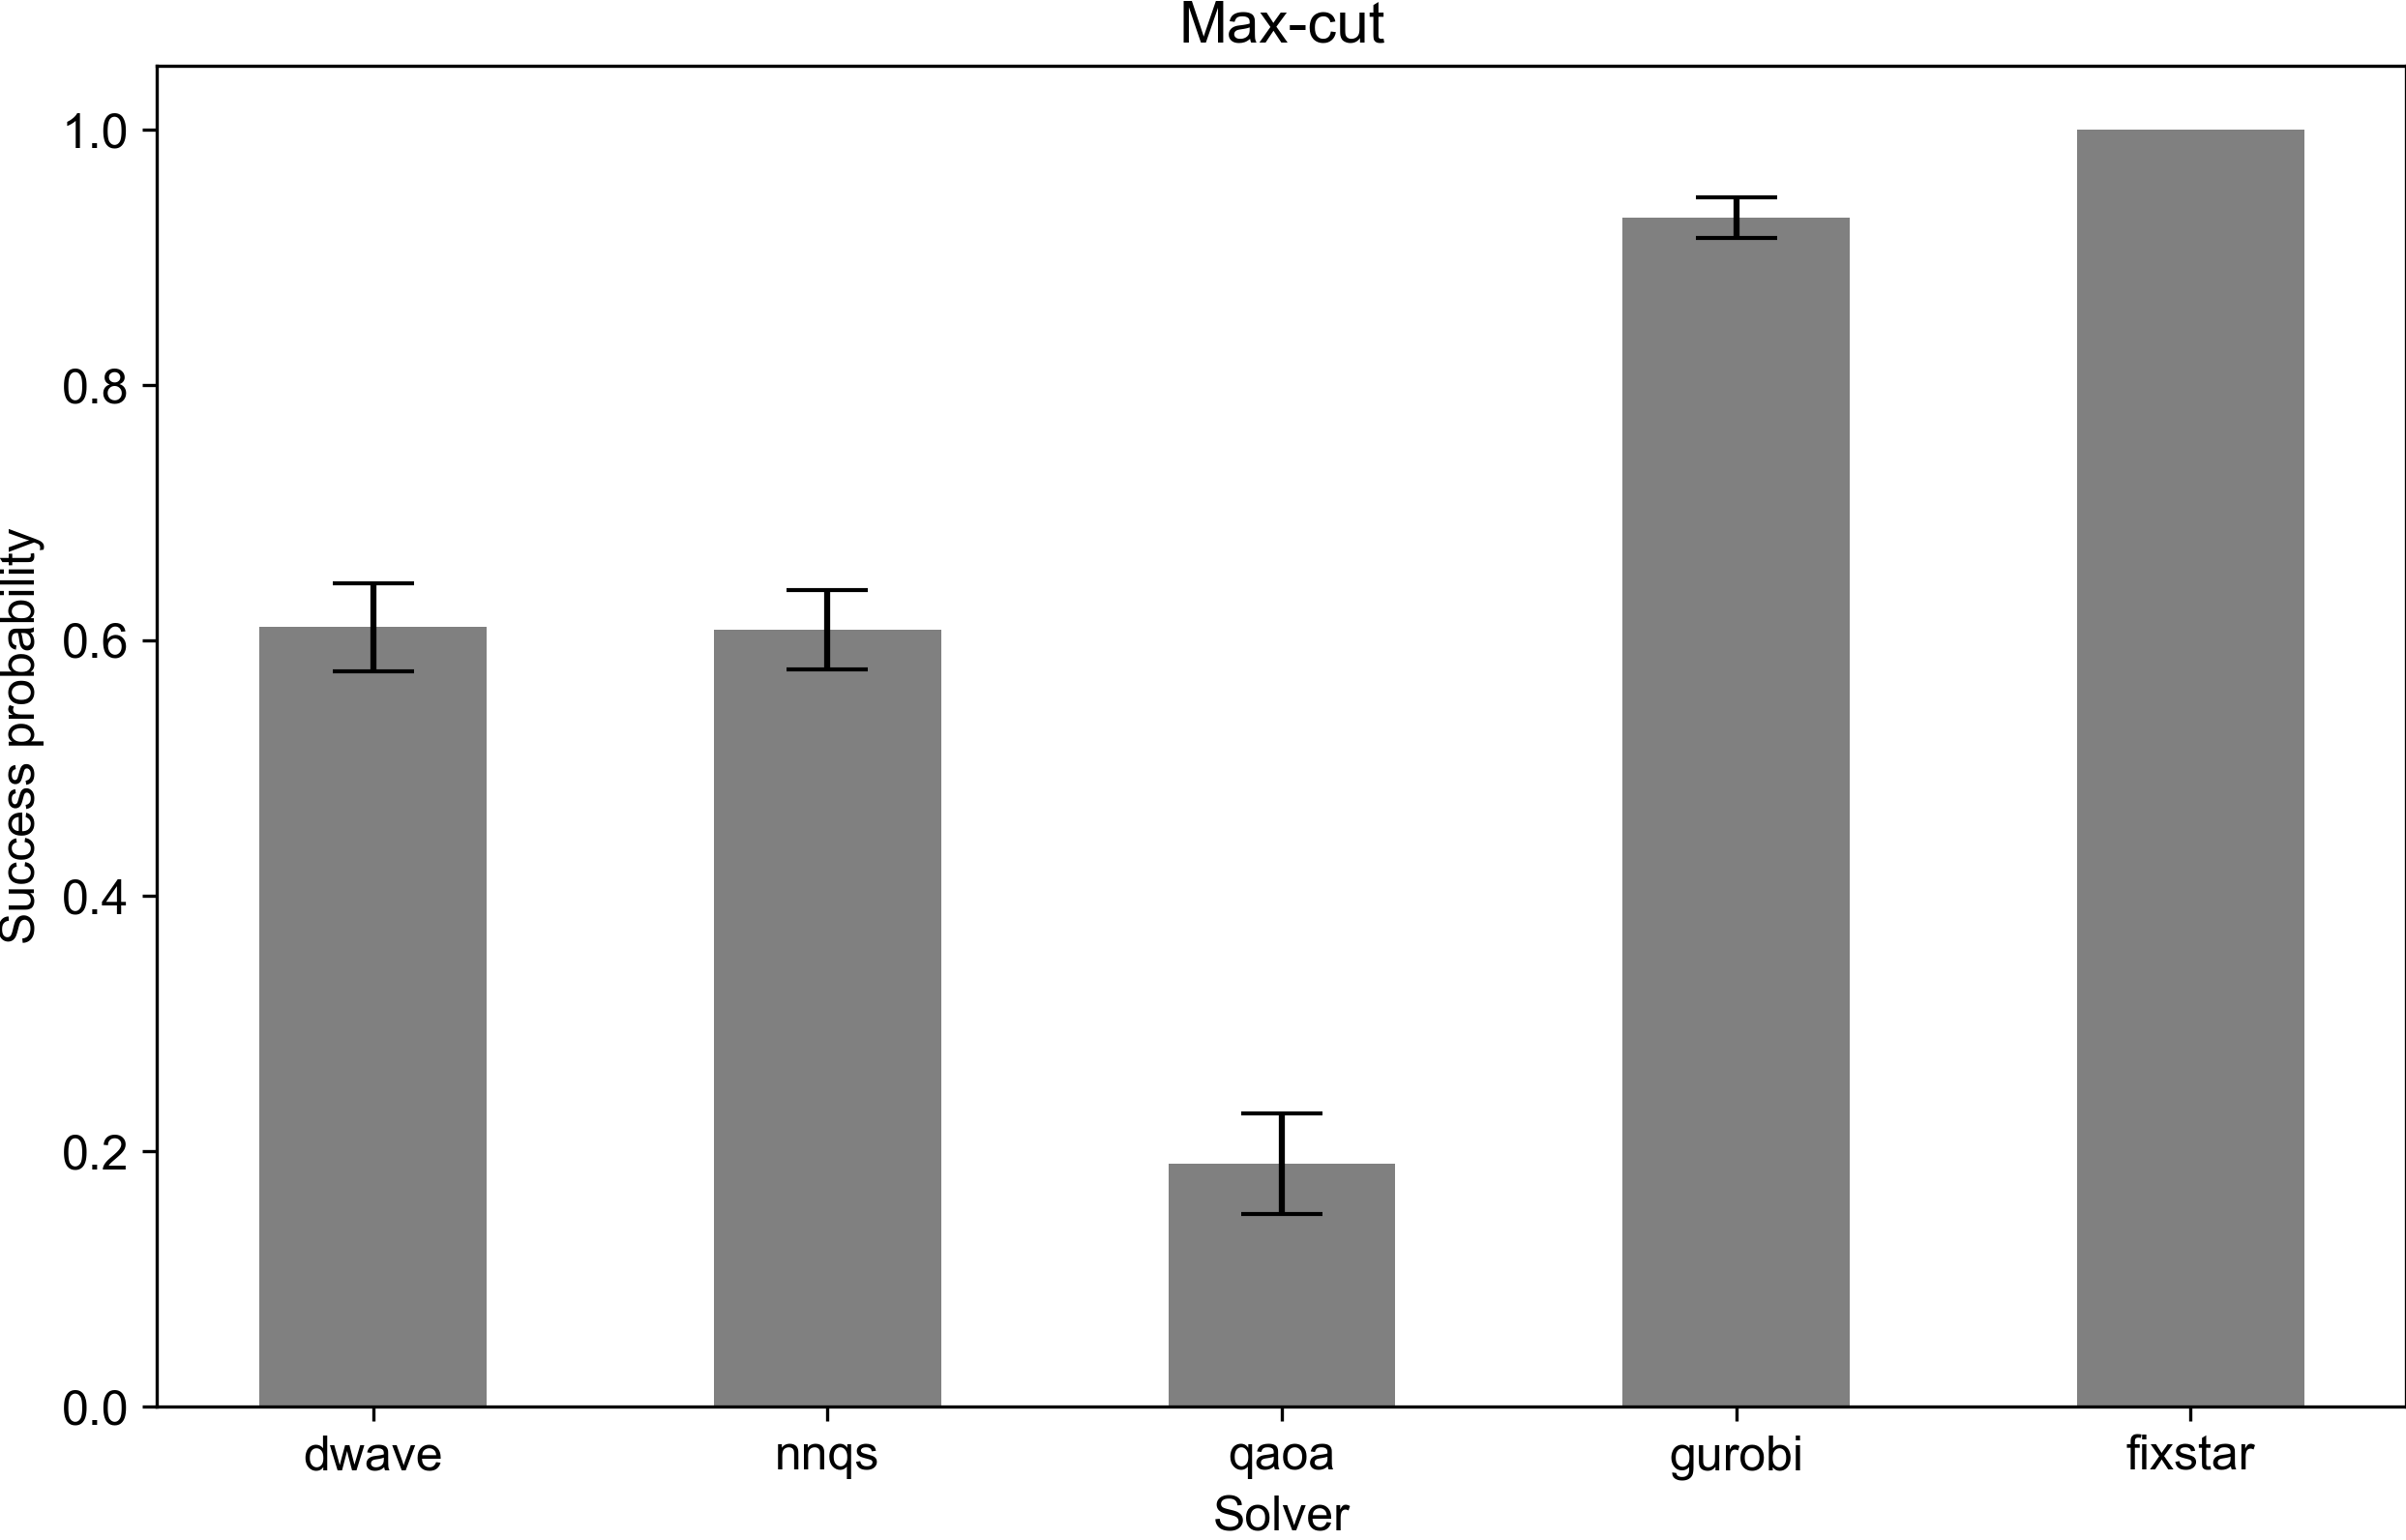
\includegraphics[width=0.4\textwidth]{images/maxcut_all_success_avg.png}}
    \caption{Average performance of different solvers for max-cut}
    \label{all-maxcut-average}
\end{figure}

The D-Wave solver performs well up to $n=30$ with a success probability of $1$, and performance drops off sharply for larger problems. The NNQS solver performs well until $n=150$, although the success probability decreases for problem sizes over $50$. The NNQS solver finds better solutions than the D-Wave solver but cannot find the best solution compared to the classical solvers. The QAOA solver performs well only for $n=10$, with performance decreases until $n=30$. The Fixstar solver consistently performs better than the GUROBI solver, while both classical solvers outperform the quantum-inspired solvers.

Overall, the NNQS has the highest average normalised energy among the three quantum-inspired solvers and has a slightly lower success probability than the D-Wave solver. The QAOA solver performs poorly in both metrics. Both classical solvers outperform the quantum-inspired solvers.

\subsection{SK model}
Performance by size for the SK model dataset is shown in \autoref{all-skmodel-size}, and average performance is shown in \autoref{all-skmodel-average}. The D-Wave solver could only solve problems up to $n=150$ due to the need for minor embedding onto the pegasus topology. The SK model is fully connected, which makes embedding difficult for large $n$. The NNQS solver could solve problems up to $n=300$. The QAOA solver is limited to problems of up to $n=30$.

\begin{figure}[!htb]
    \centering
    \subfloat[Normalized energy]{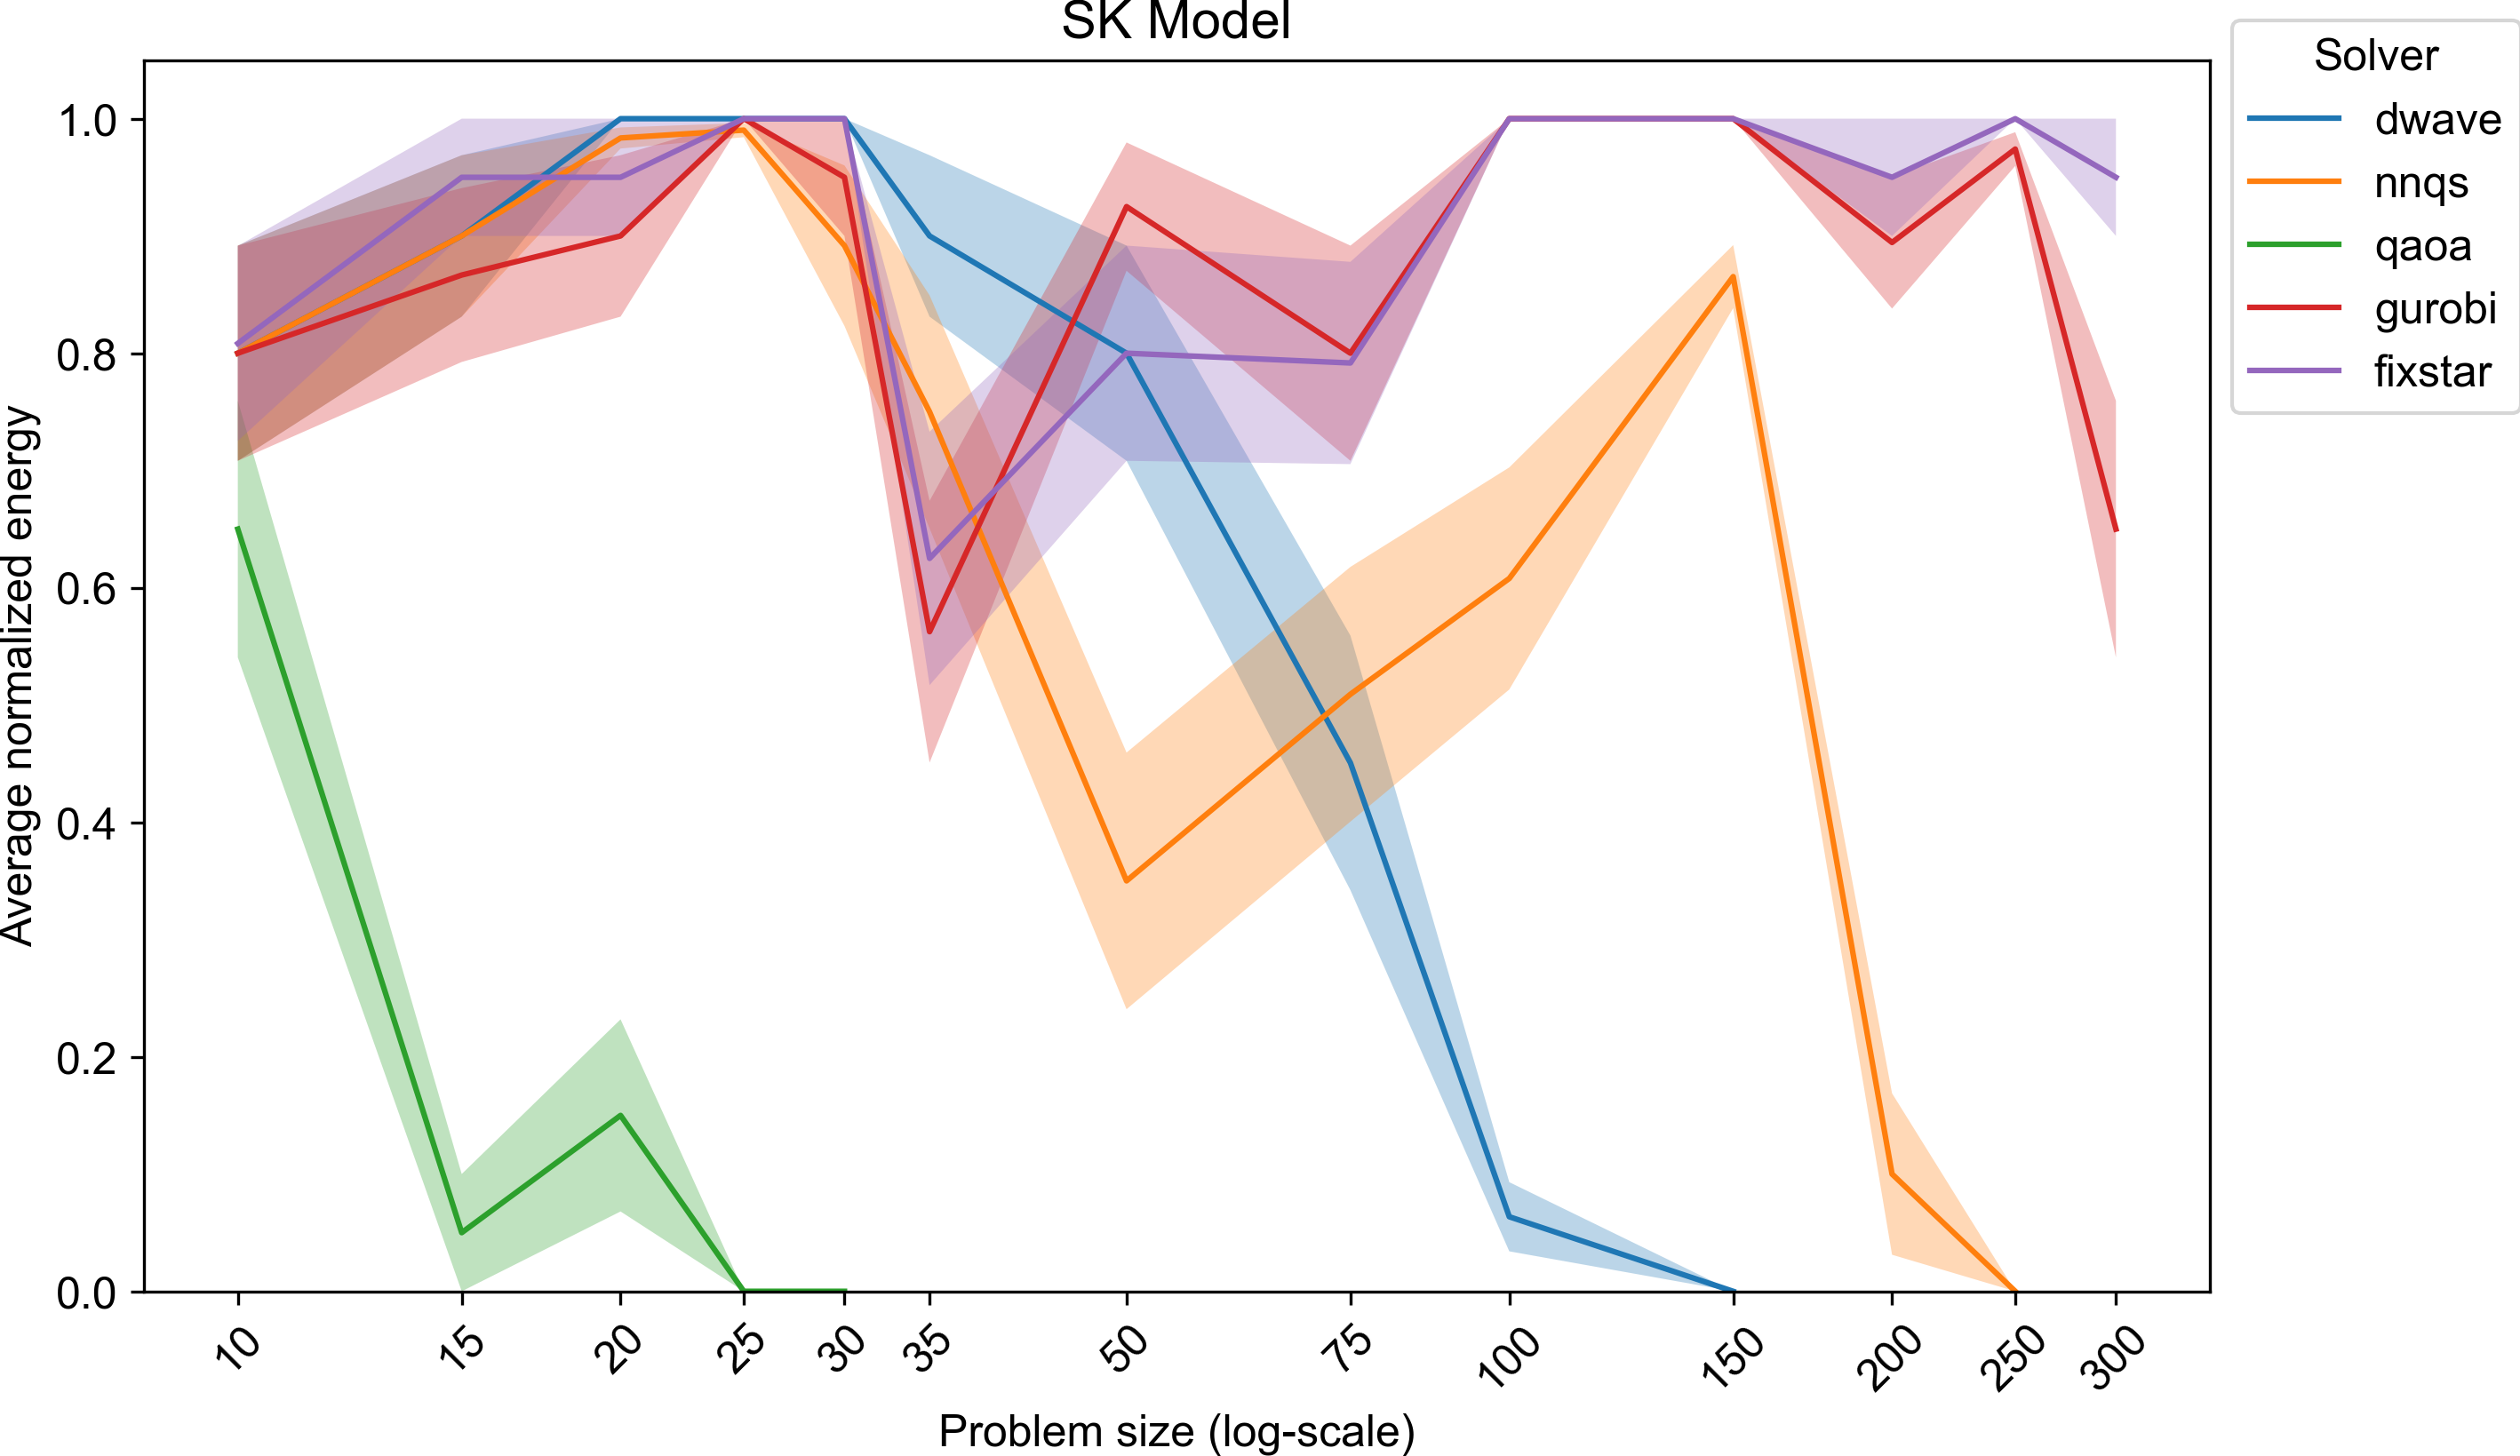
\includegraphics[width=0.5\textwidth]{images/skmodel_all_size.png}}%\hfill
    \subfloat[Success probability]{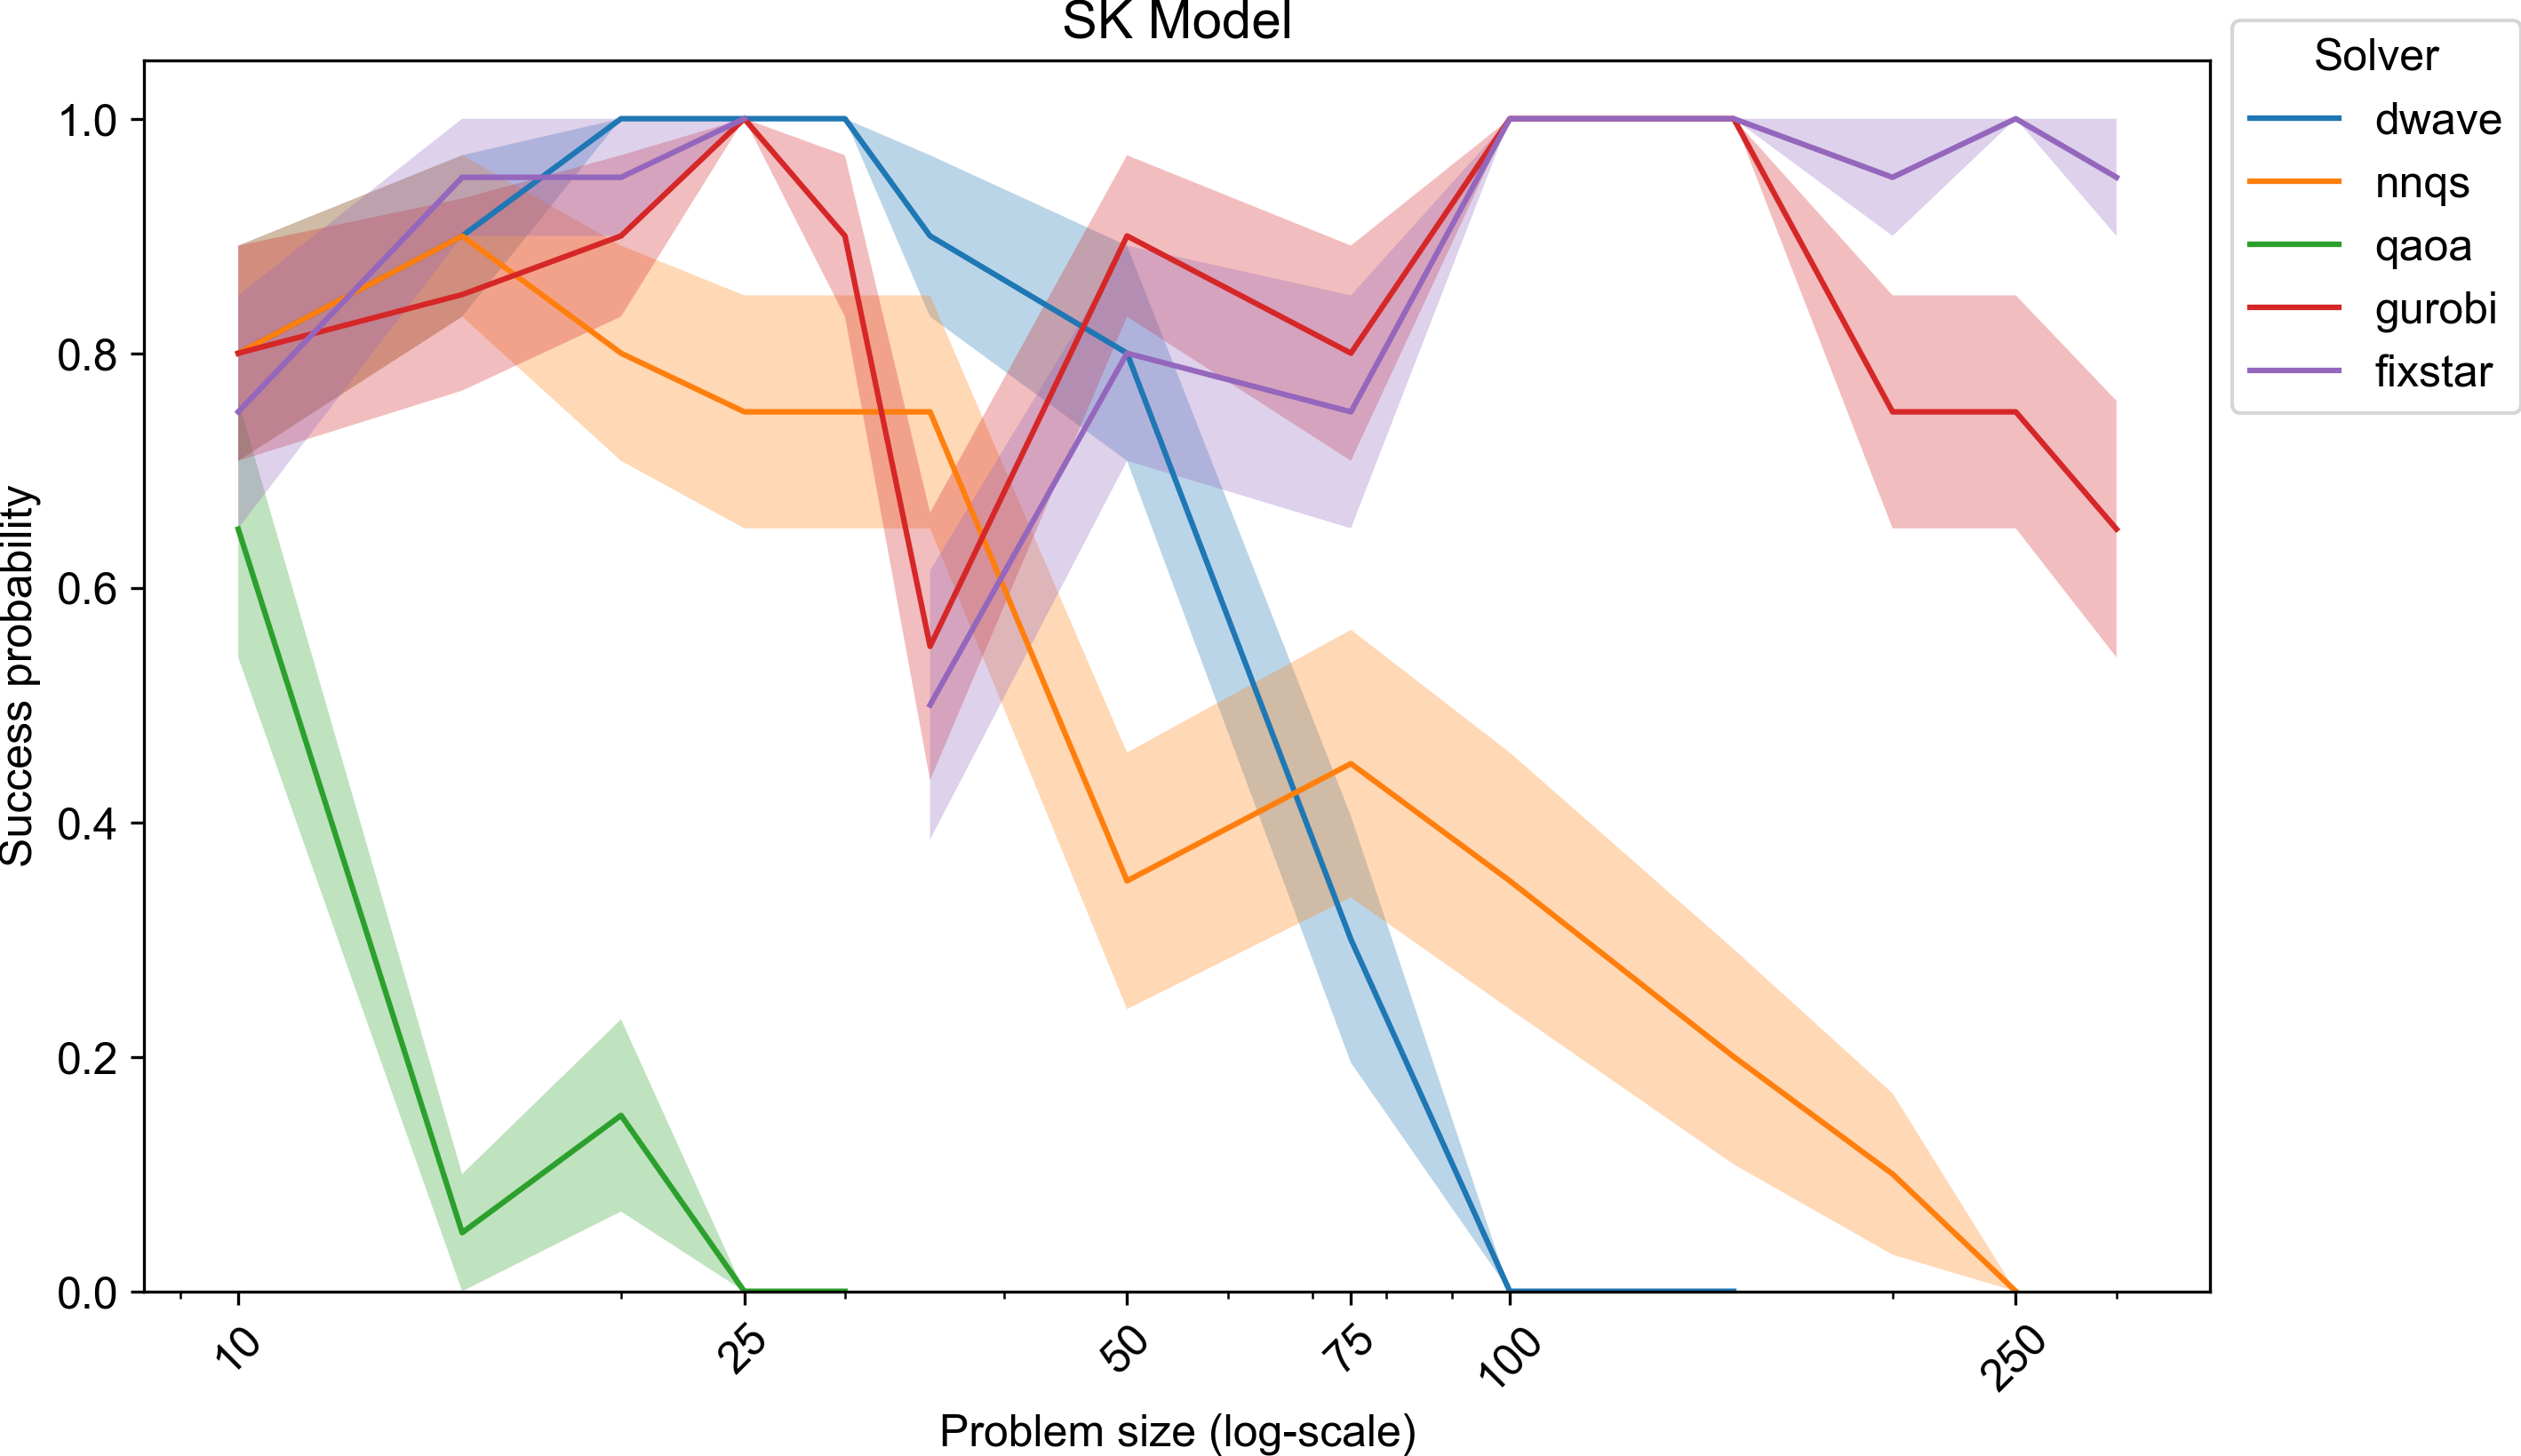
\includegraphics[width=0.5\textwidth]{images/skmodel_all_success_size.png}}
    \caption{Performance of different solvers for SK model by problem size}
    \label{all-skmodel-size}
\end{figure}

\begin{figure}[!htb]
    \centering
    \subfloat[Normalized energy]{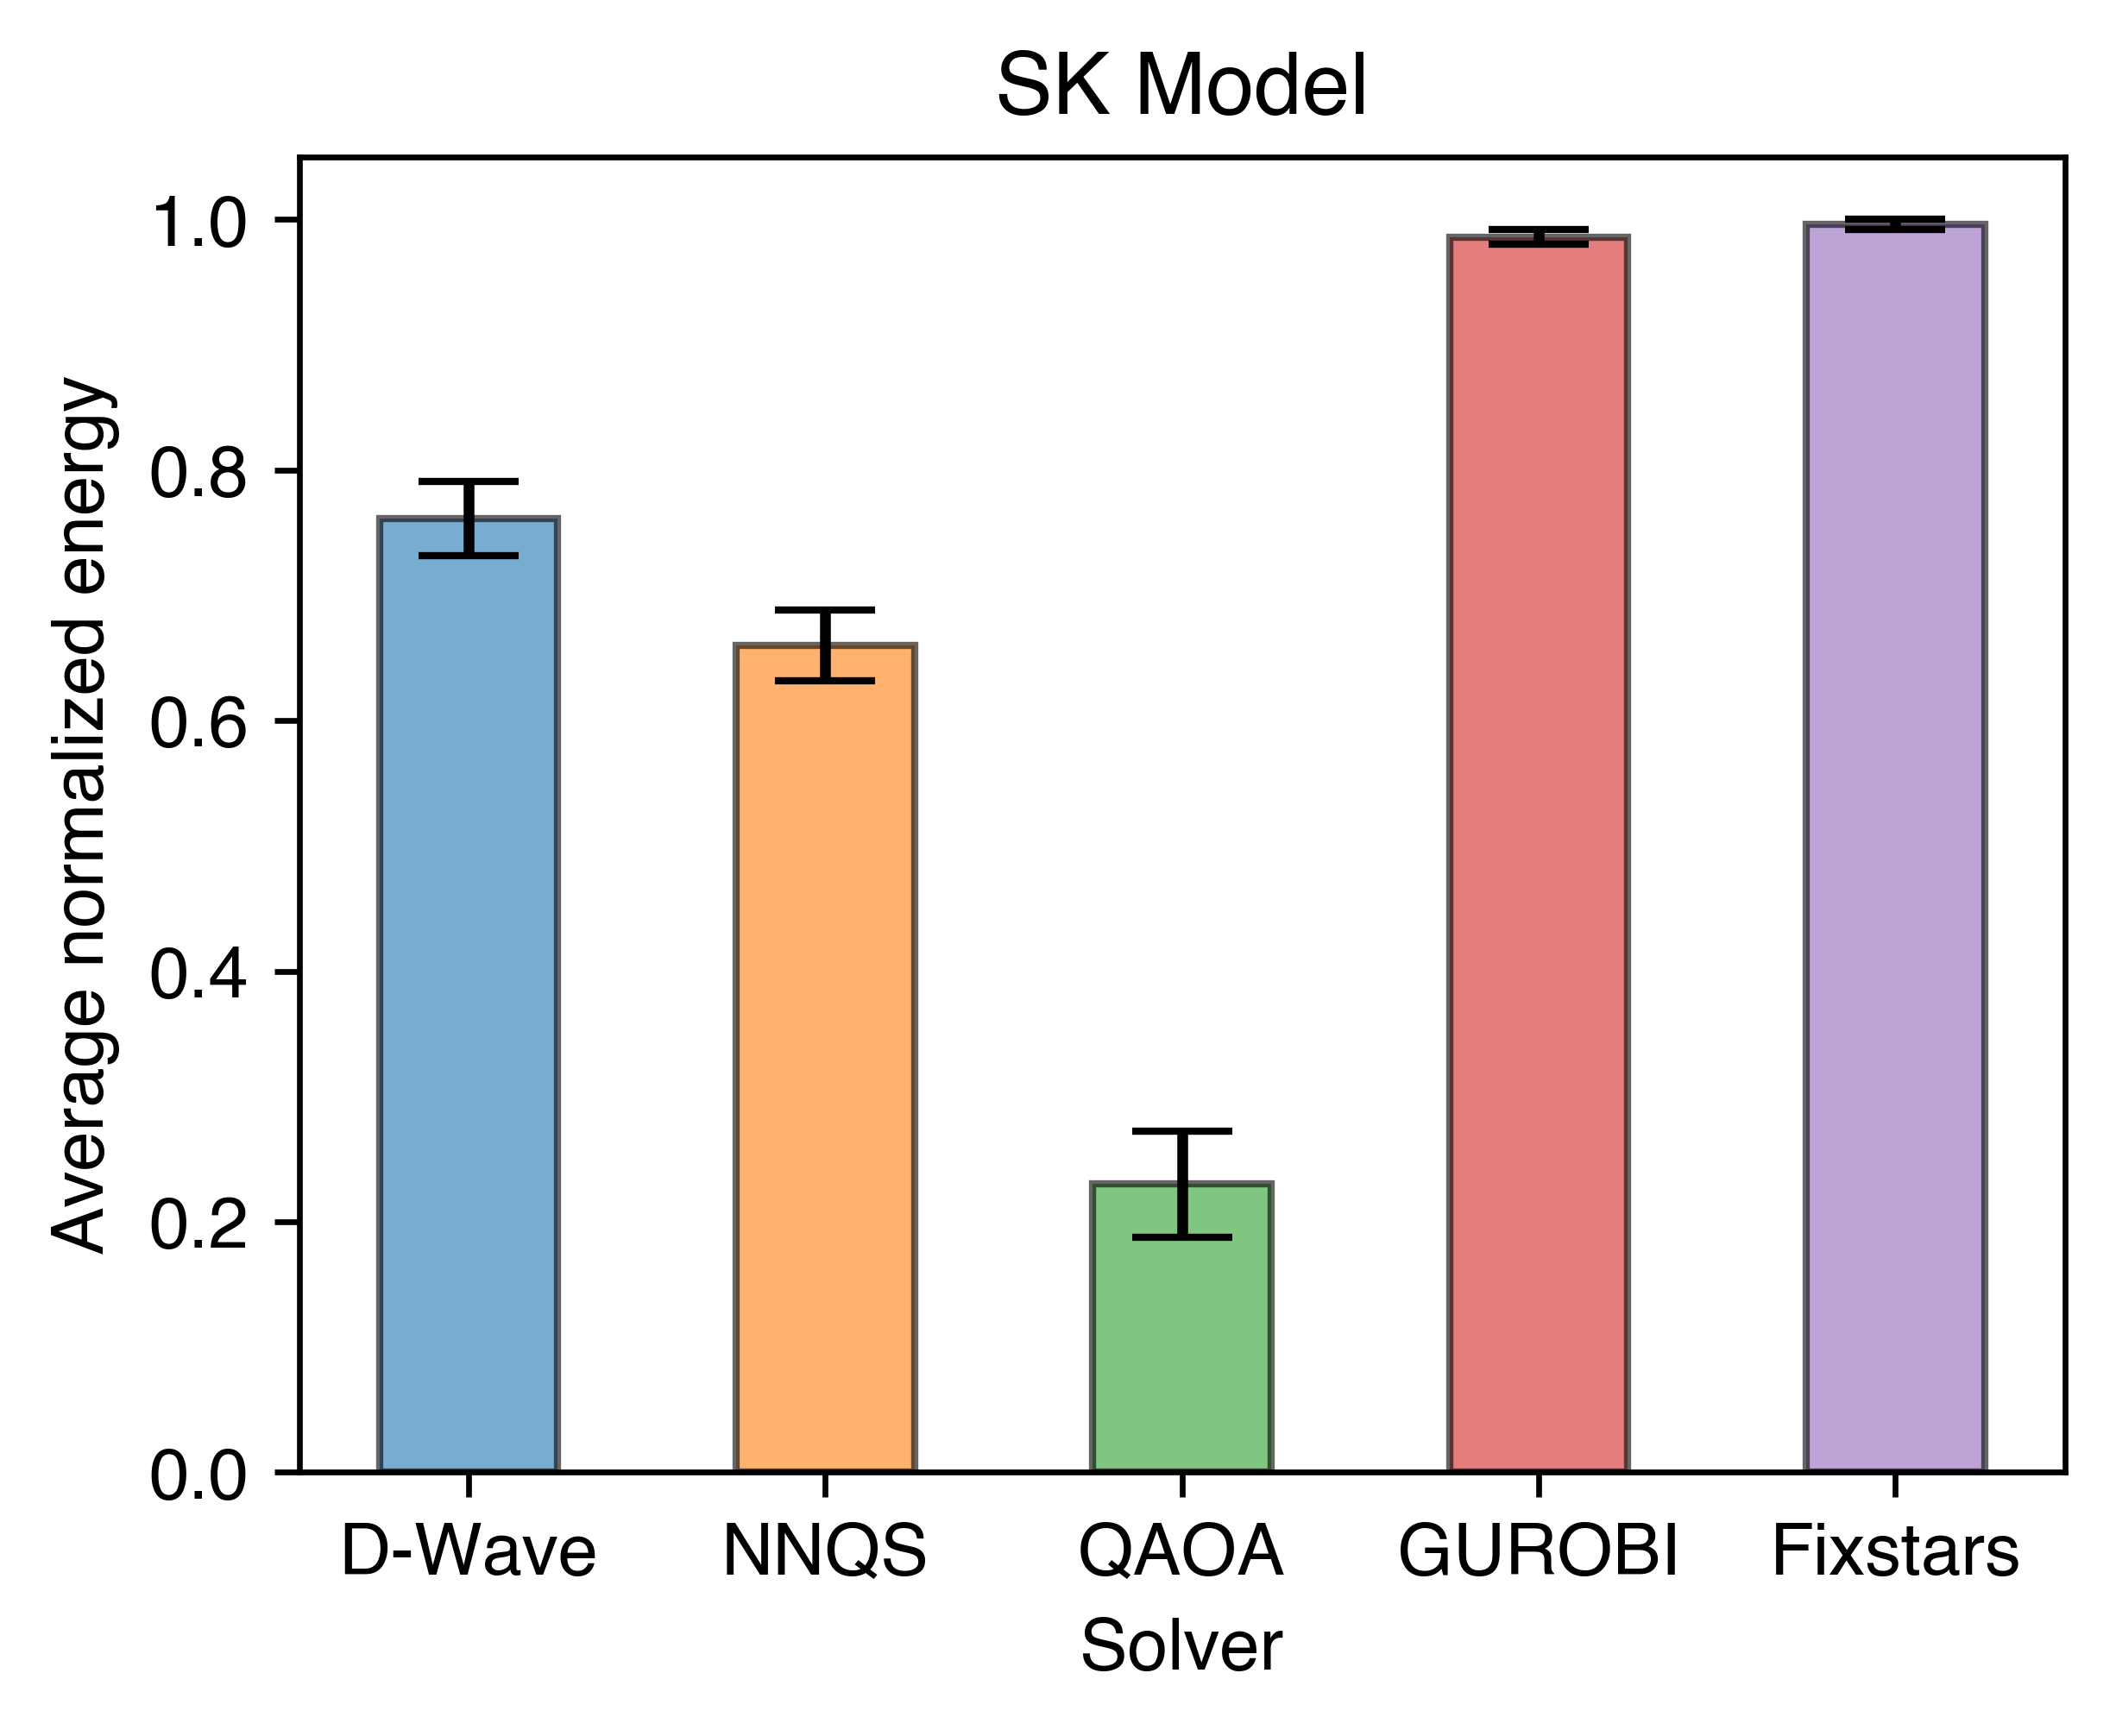
\includegraphics[width=0.4\textwidth]{images/skmodel_all_avg.png}}\hspace{30px}
    \subfloat[Success probability]{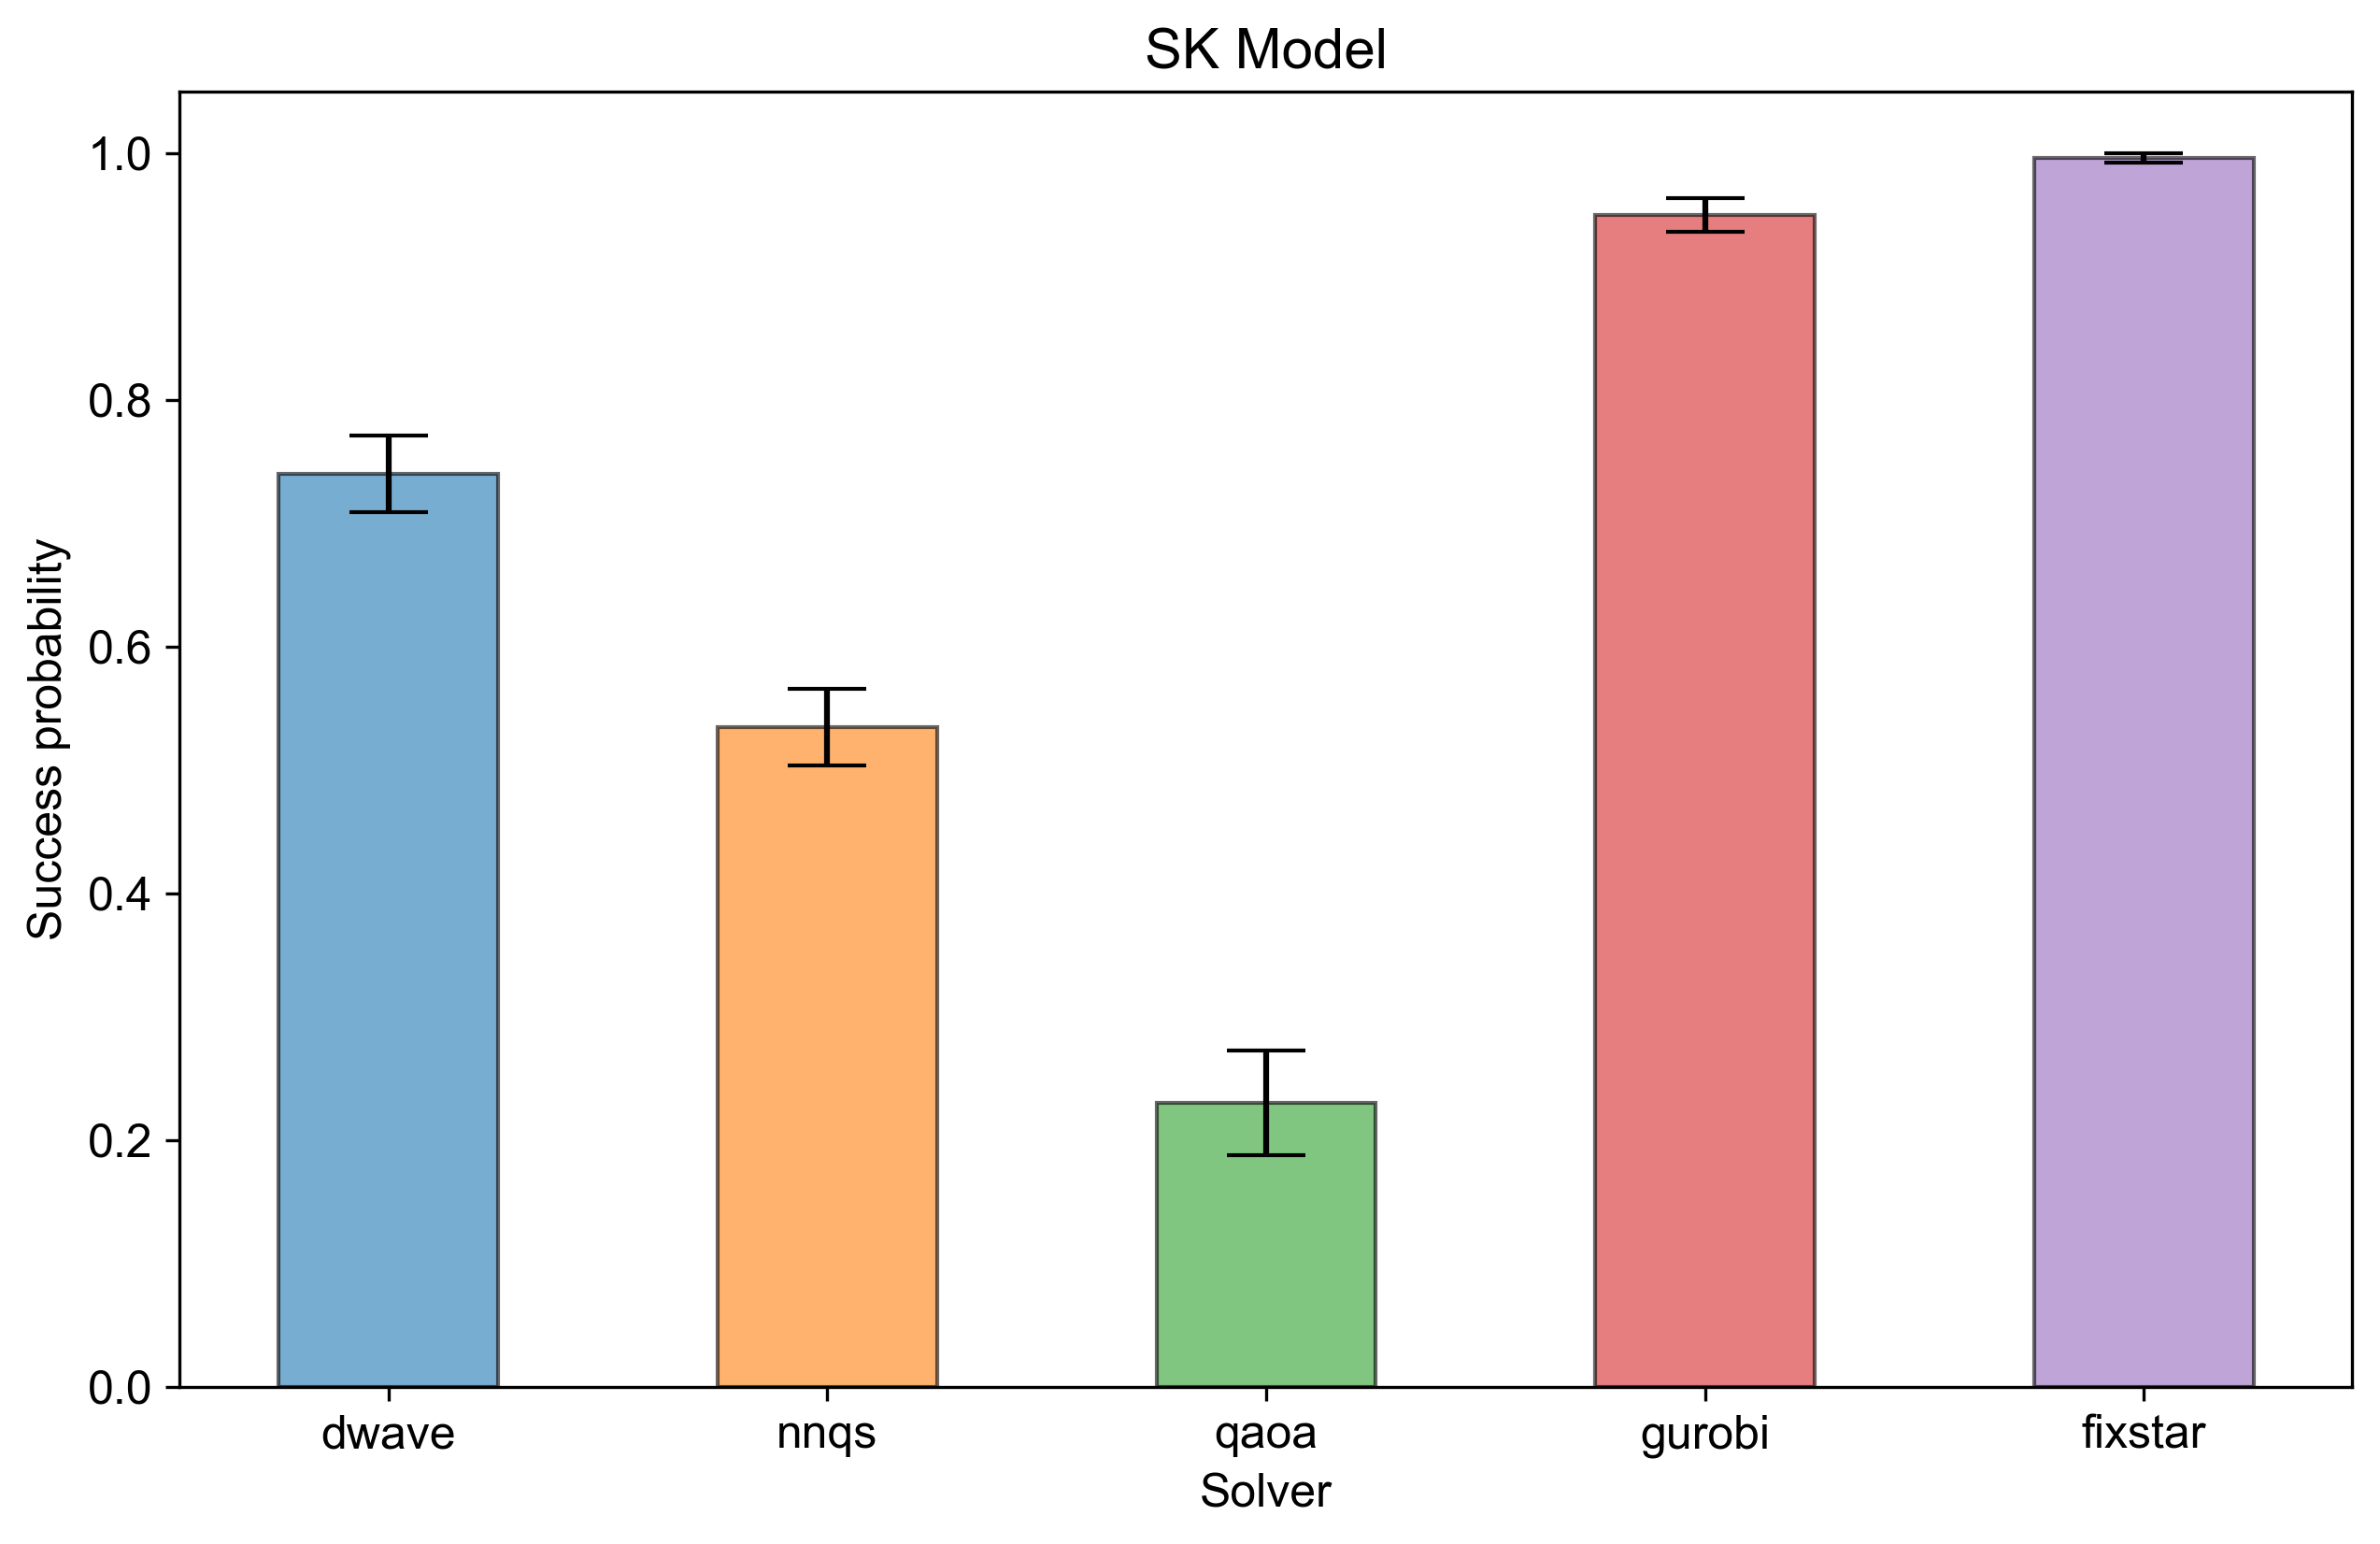
\includegraphics[width=0.4\textwidth]{images/skmodel_all_success_avg.png}}
    \caption{Average performance of different solvers for SK model}
    \label{all-skmodel-average}
\end{figure}

The D-Wave solver performs well up to $n=50$ with a success probability of $1$. For larger problem sizes, the performance of the D-Wave solver drops off sharply. The NNQS solver performs well up to $n=15$, with the success probability gradually decreasing with increasing problem size. The QAOA solver performs poorly for all problem sizes, possibly as the SK model presents a more difficult optimisation problem. Between the classical solvers, the Fixstars QUBO solver performs better than the GUROBI optimiser except for $n=35$. However, this is likely due to variance in the randomly generated dataset. Both classical solvers generally outperform the quantum-inspired solvers.

Overall, the D-Wave annealer has the highest average normalised energy and success probability among the three quantum-inspired solvers. The NNQS is slightly worse in both metrics, while the QAOA solver performs poorly for both metrics. Both classical solvers outperform the quantum-inspired solvers.

\section{Time-Constrained Solver Comparison}
We also measured the average runtime for each solver by problem type and size shown in \autoref{results:timeaverage}. Runtimes split by problem type can be found in \autoref{appendix:timesizegraph}

\begin{figure}[!htb]
    \centering
    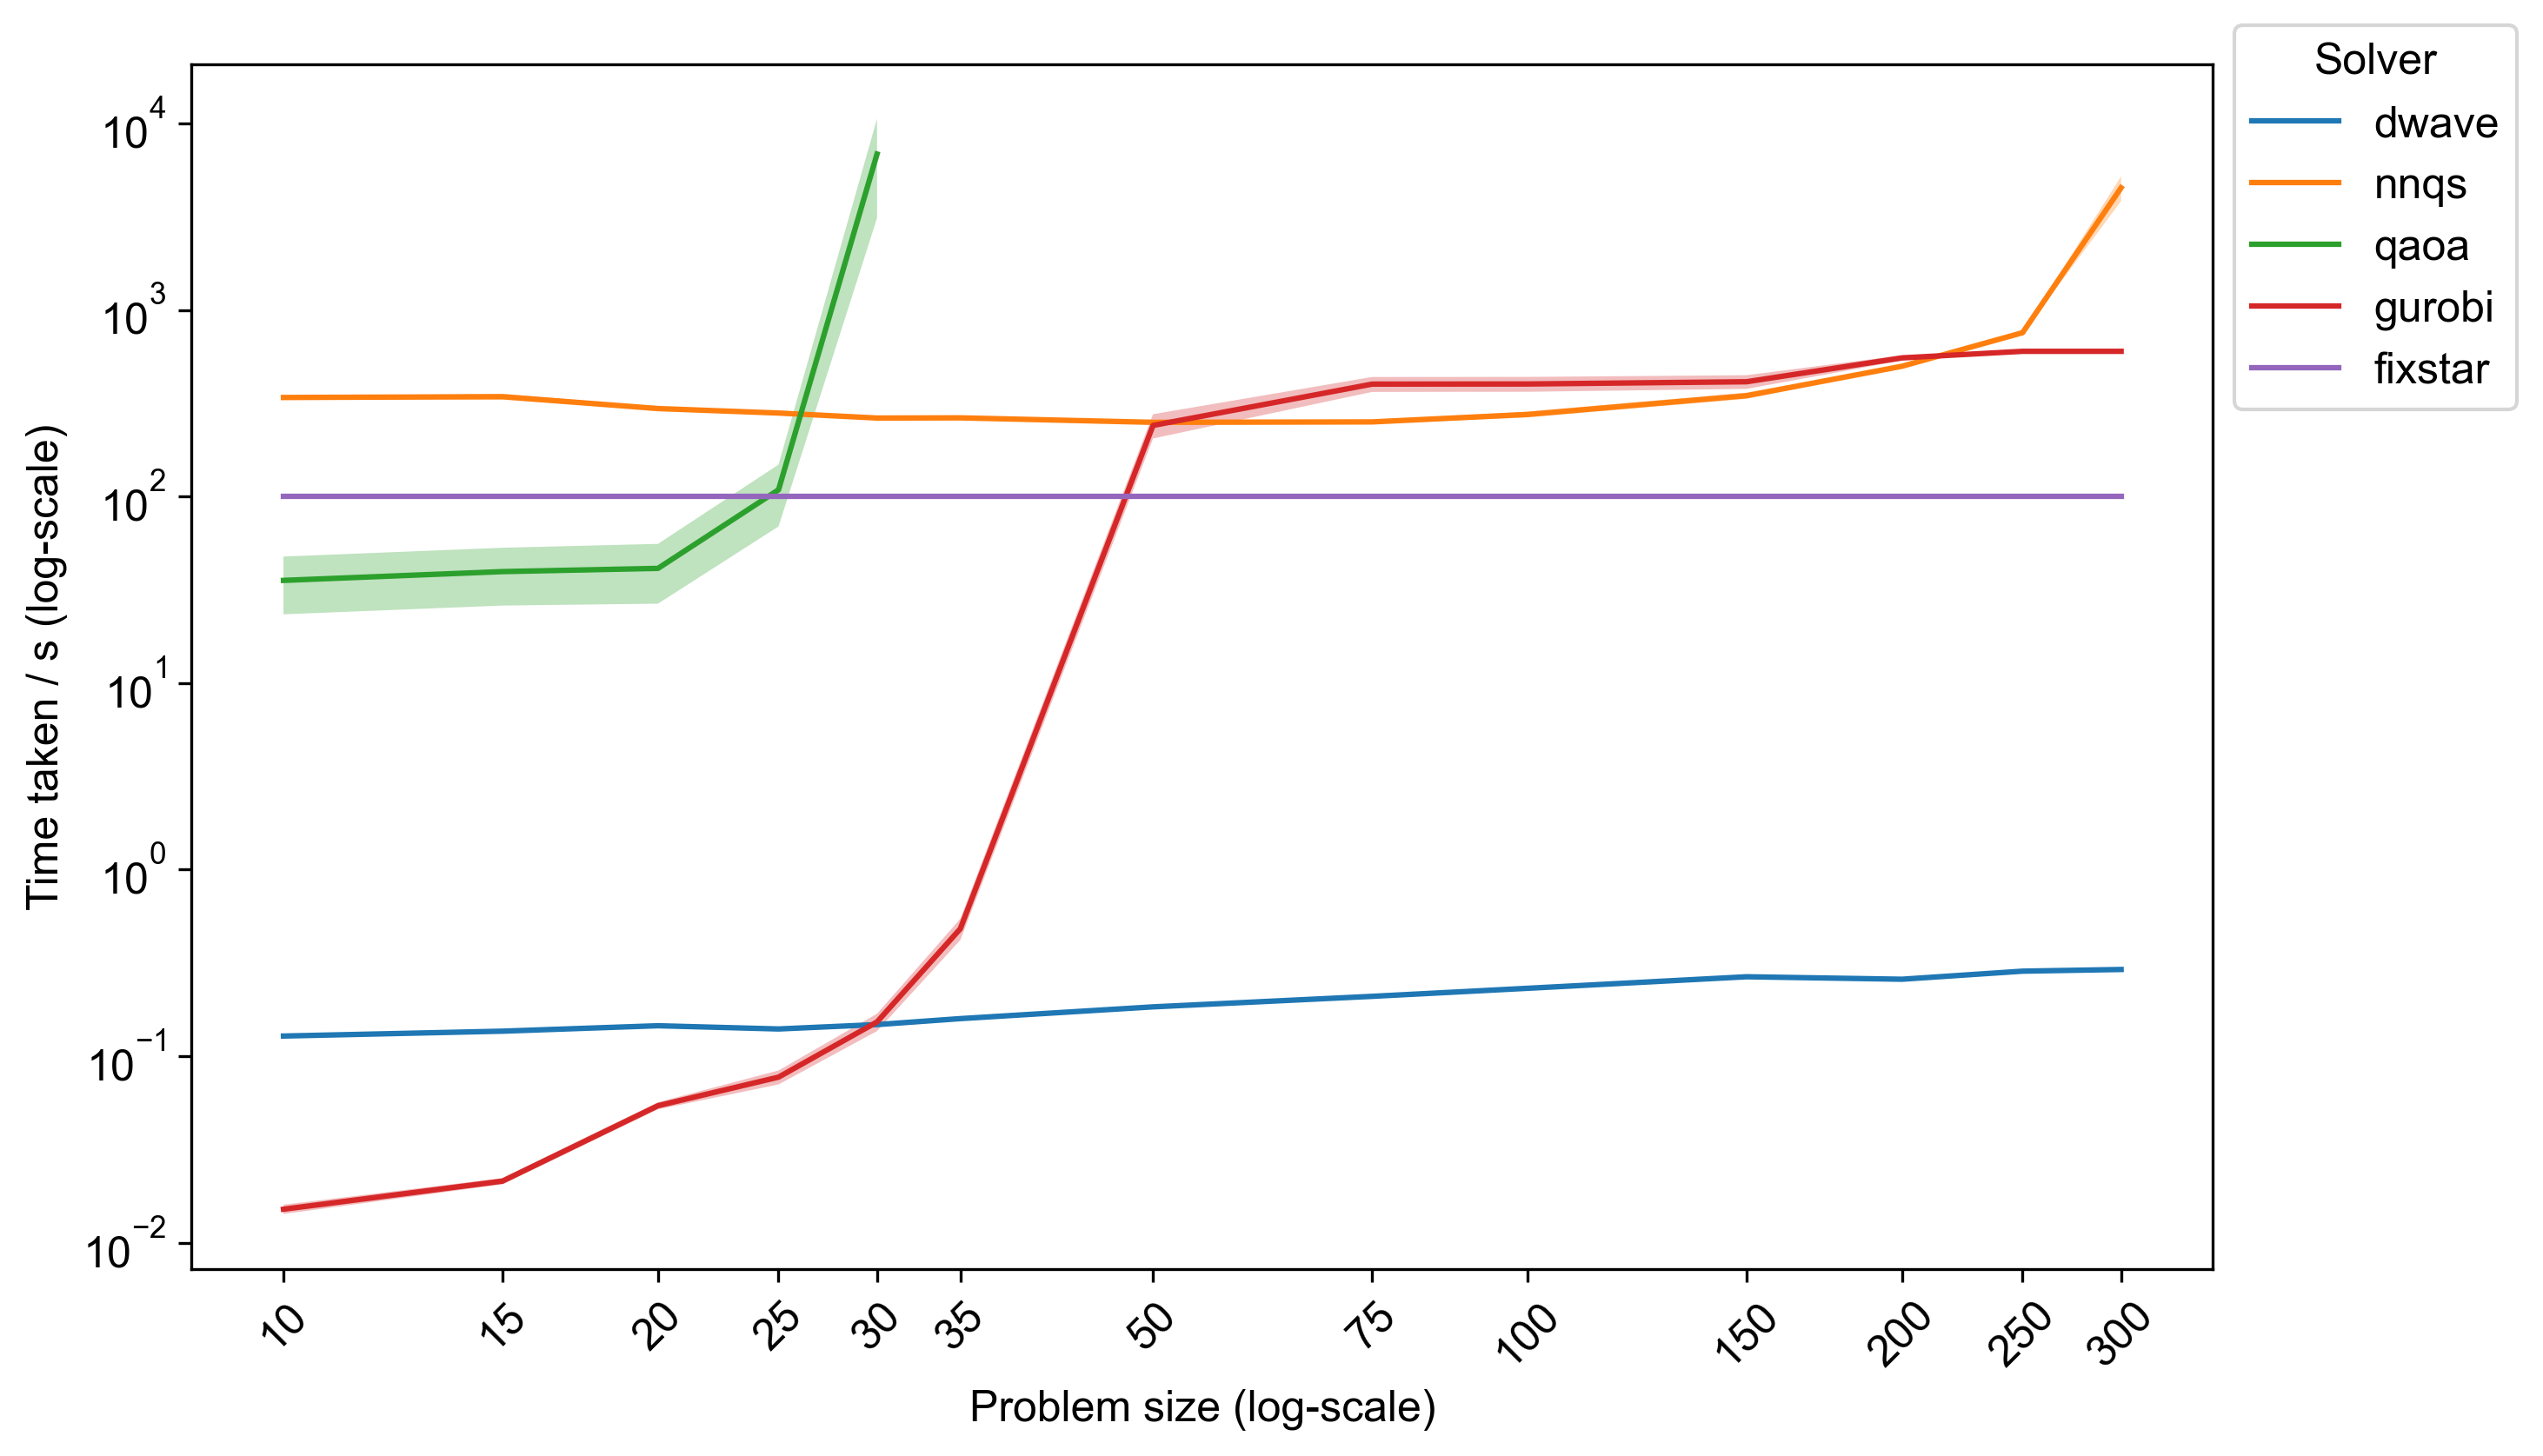
\includegraphics[width=0.6\textwidth]{images/all_time_average.png}
    \caption{Average runtime taken by different solvers for QUBO problems by size. Both problem size and average runtime are plotted in log scale.}
    \label{results:timeaverage}
\end{figure}

The runtime of the D-Wave solver increases approximately linearly from $0.128\si{\second}$ for $n=10$ to $0.184\si{\second}$ for $n=50$ and $0.292\si{\second}$ for $n=300$. The runtime of the NNQS solver remains from $250\si{\second}$ to $350\si{\second}$ for $n$ between $10$ and $200$ but increases sharply for $n \geq 250$, which could be due to memory issues with the GPU or a longer sampling time. The QAOA solver's runtime remains stable from $n=10$ to $n=20$ at around $38 \si{\second}$. However, it increases rapidly to $6847 \si{\second}$ at $n=30$ due to the need for many more iterations for the parameters to converge and greater computational resources for the simulation.

The GUROBI optimiser was set with a maximum time limit of $600 \si{\second}$ but could finish solving before the time limit for most problems with $n \leq 35$. The Fixstar solver was configured with a time limit of $100 \si{\second}$, the maximum possible duration, with each solve utilising the entire time limit.

Since the D-Wave solver seems to be the most promising quantum-inspired solver, we conducted an additional experiment where the runtimes were matched. Using the average runtime of the D-Wave solver, we measured the performance of the D-Wave solver against the GUROBI and Fixstar solvers to see if the D-Wave solver could outperform the classical solvers when limited to the same runtime. The classical solvers were run with a runtime limit equal to the average runtime by the D-Wave solver for problems of equivalent type and size shown in \autoref{results:averageruntimedwave}.

\begin{table}[!htb]
    \centering
    \resizebox{\textwidth}{!}{%
    \begin{tabular}{lrrrrrrrrrrrrr} \toprule
        $n$ & 10 & 15 & 20 & 25 & 30 & 35 & 50 & 75 & 100 & 150 & 200 & 250 & 300 \\ \midrule
        NAE3SAT & 0.133 & 0.135 & 0.141 & 0.149 & 0.138 & 0.156 & 0.173 & 0.184 & 0.201 & 0.243 & 0.259 & 0.286 & 0.292 \\
        Max-cut & 0.127 & 0.136 & 0.1560 & 0.130 & 0.155 & 0.160 & 0.183 & 0.223 & 0.247 & 0.278 & - & - & - \\
        SK model & 0.125 & 0.137 & 0.140 & 0.140 & 0.150 & 0.161 & 0.195 & 0.221 & 0.245 & 0.278 & - & - & - \\ \bottomrule
    \end{tabular}}
    \caption{Average runtime (seconds) of the D-Wave solver by problem type and size. Dashes indicate that the D-Wave solver could not embed problems of that size.}
    \label{results:averageruntimedwave}
\end{table}

The average performance is shown in \autoref{all-time-size}. For each problem type, the performance of the GUROBI solver drops before the D-Wave solver, and there are problem types and sizes where the D-Wave solver outperforms the GUROBI solver. The D-Wave solver outperforms the GUROBI solver for the NAE3SAT problems with $n=50, 75$, max-cut problems with $n=30, 35$, and the SK model with $n=20, 35$. However, when the problem sizes increase even further, the D-Wave solver underperforms the classical solvers, possibly due to the increased noise of the quantum annealer. The Fixstar solver remains the best-performing solver across all problem types for almost all sizes, even when the runtime is matched with the D-Wave solver. The results show that the D-Wave solver can outperform the GUROBI solver for specific problem sizes when the runtime is matched, a new result that has not been shown in the literature. 

\begin{figure}[!htb]
    \centering
    \subfloat[NAE3SAT]{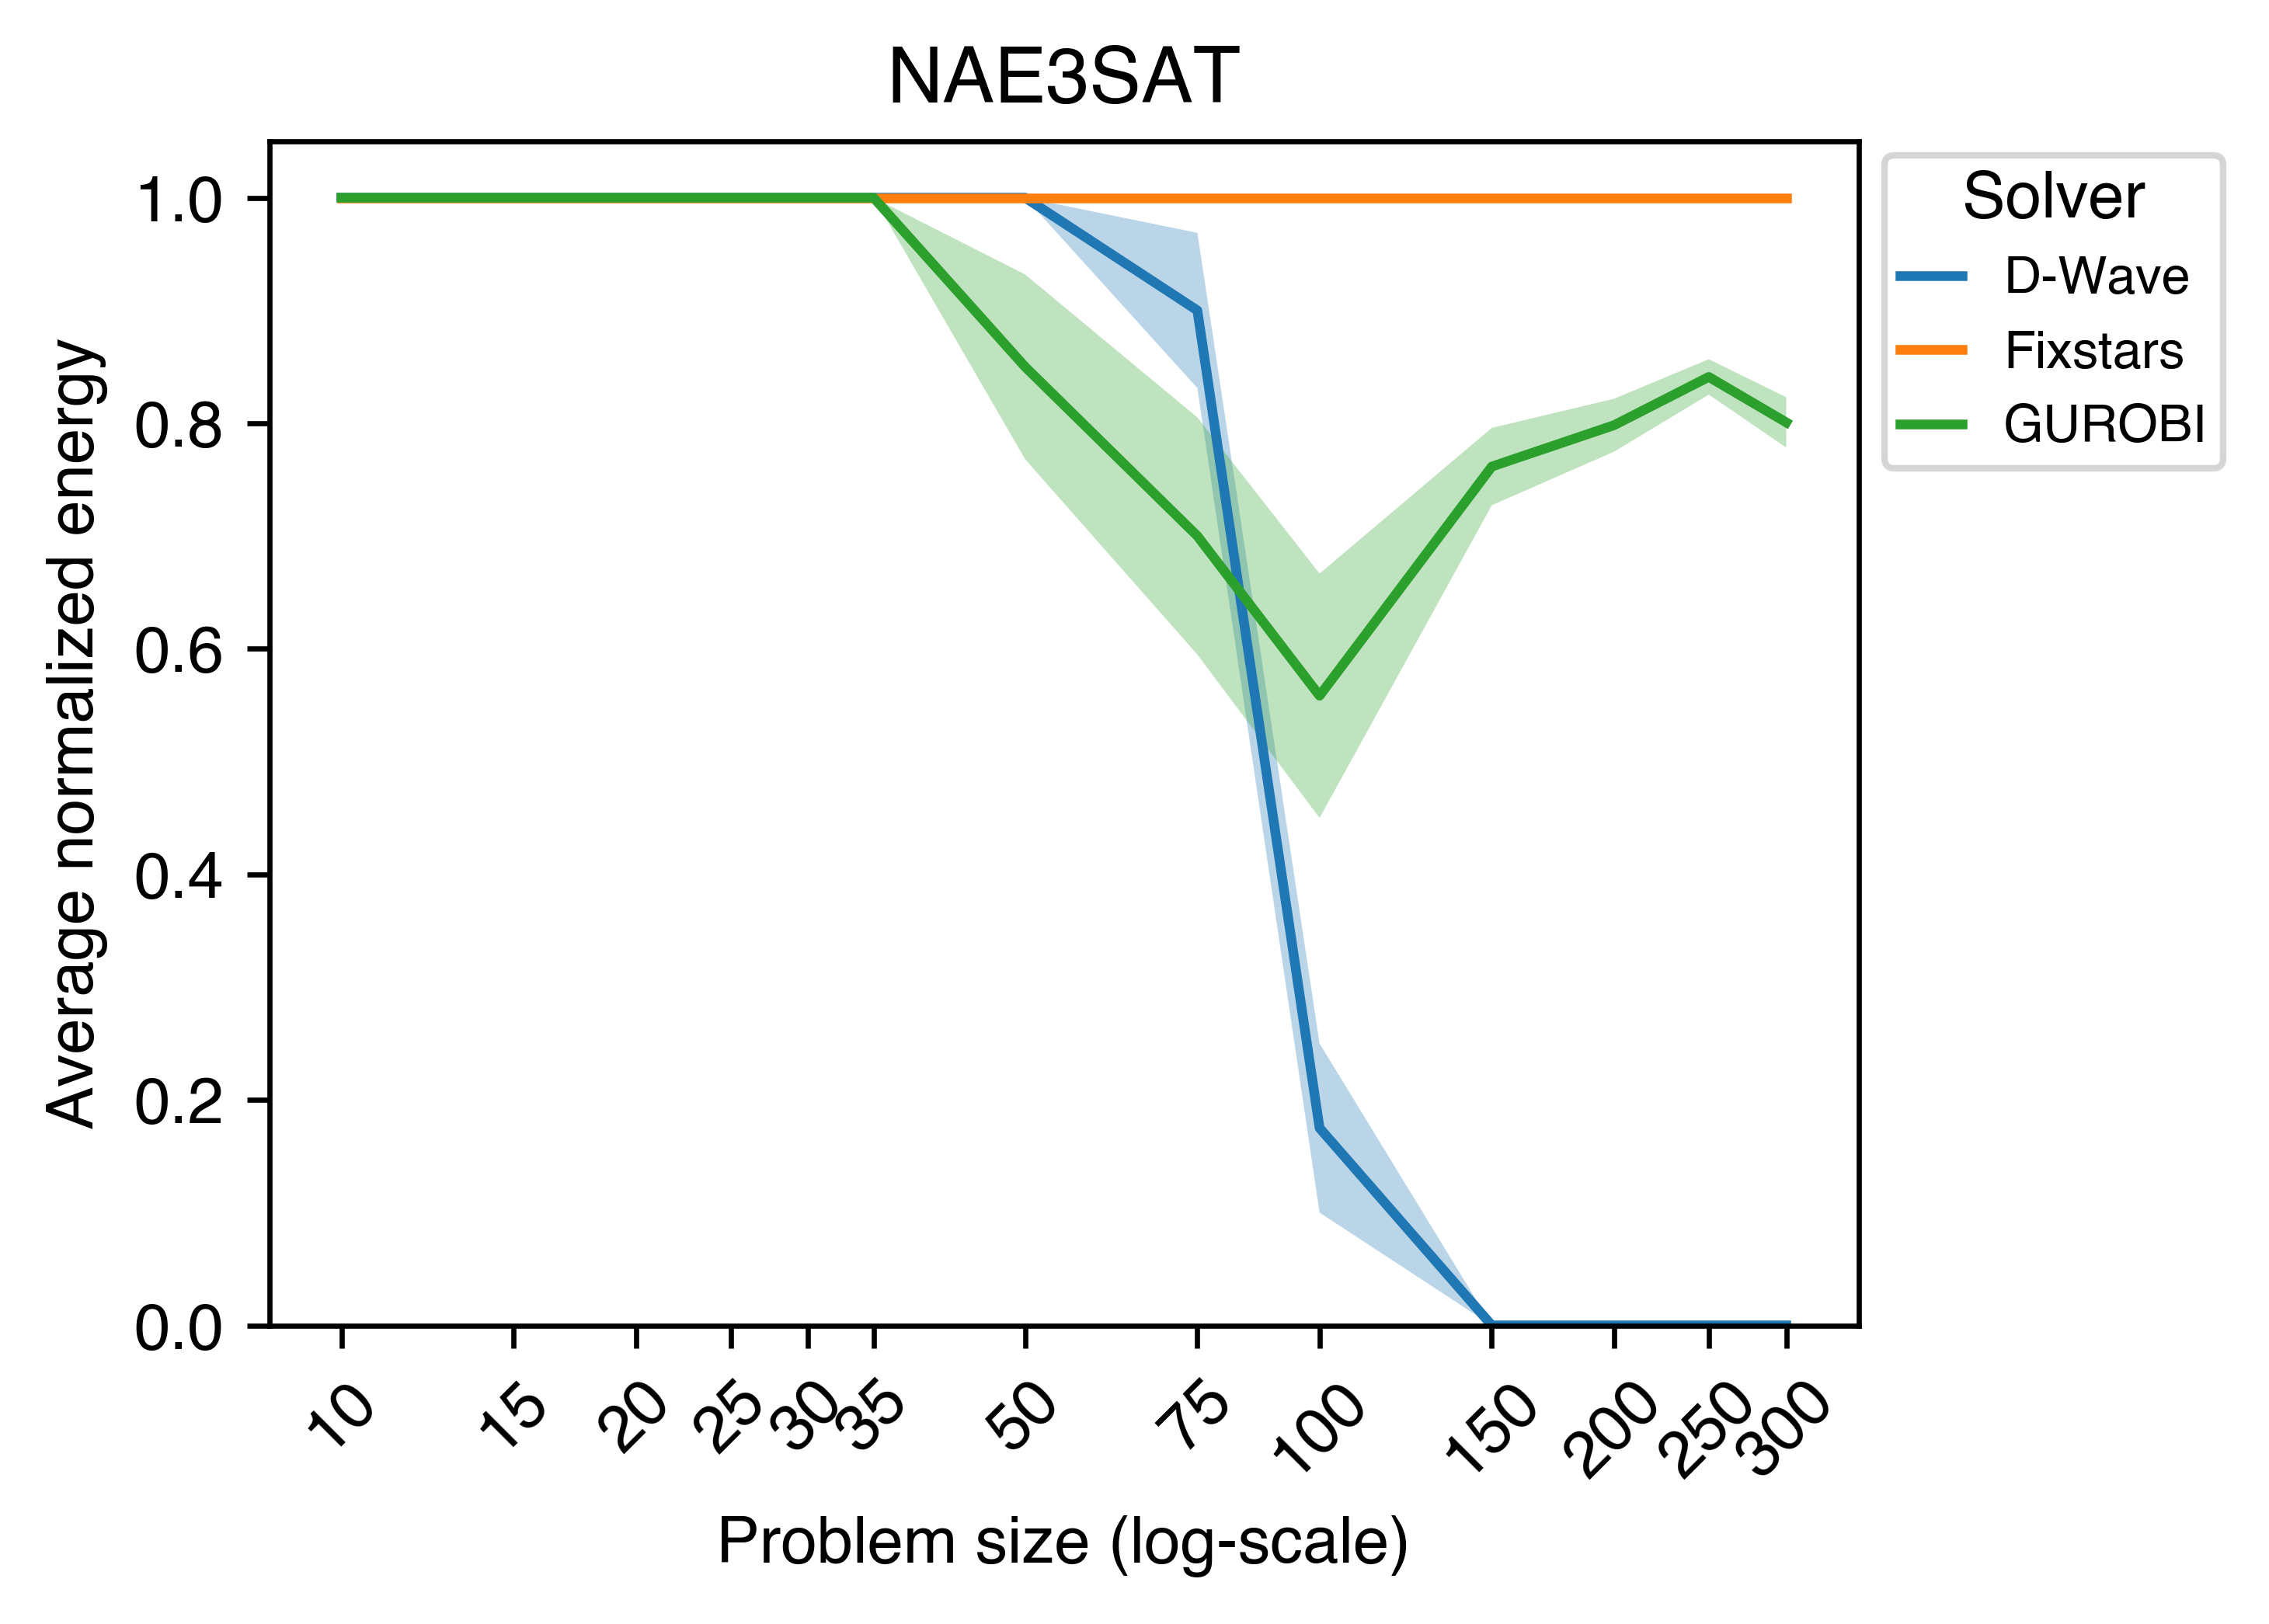
\includegraphics[width=0.5\textwidth]{images/nae3sat_timing_size.png}}\hfill
    \subfloat[Max-cut]{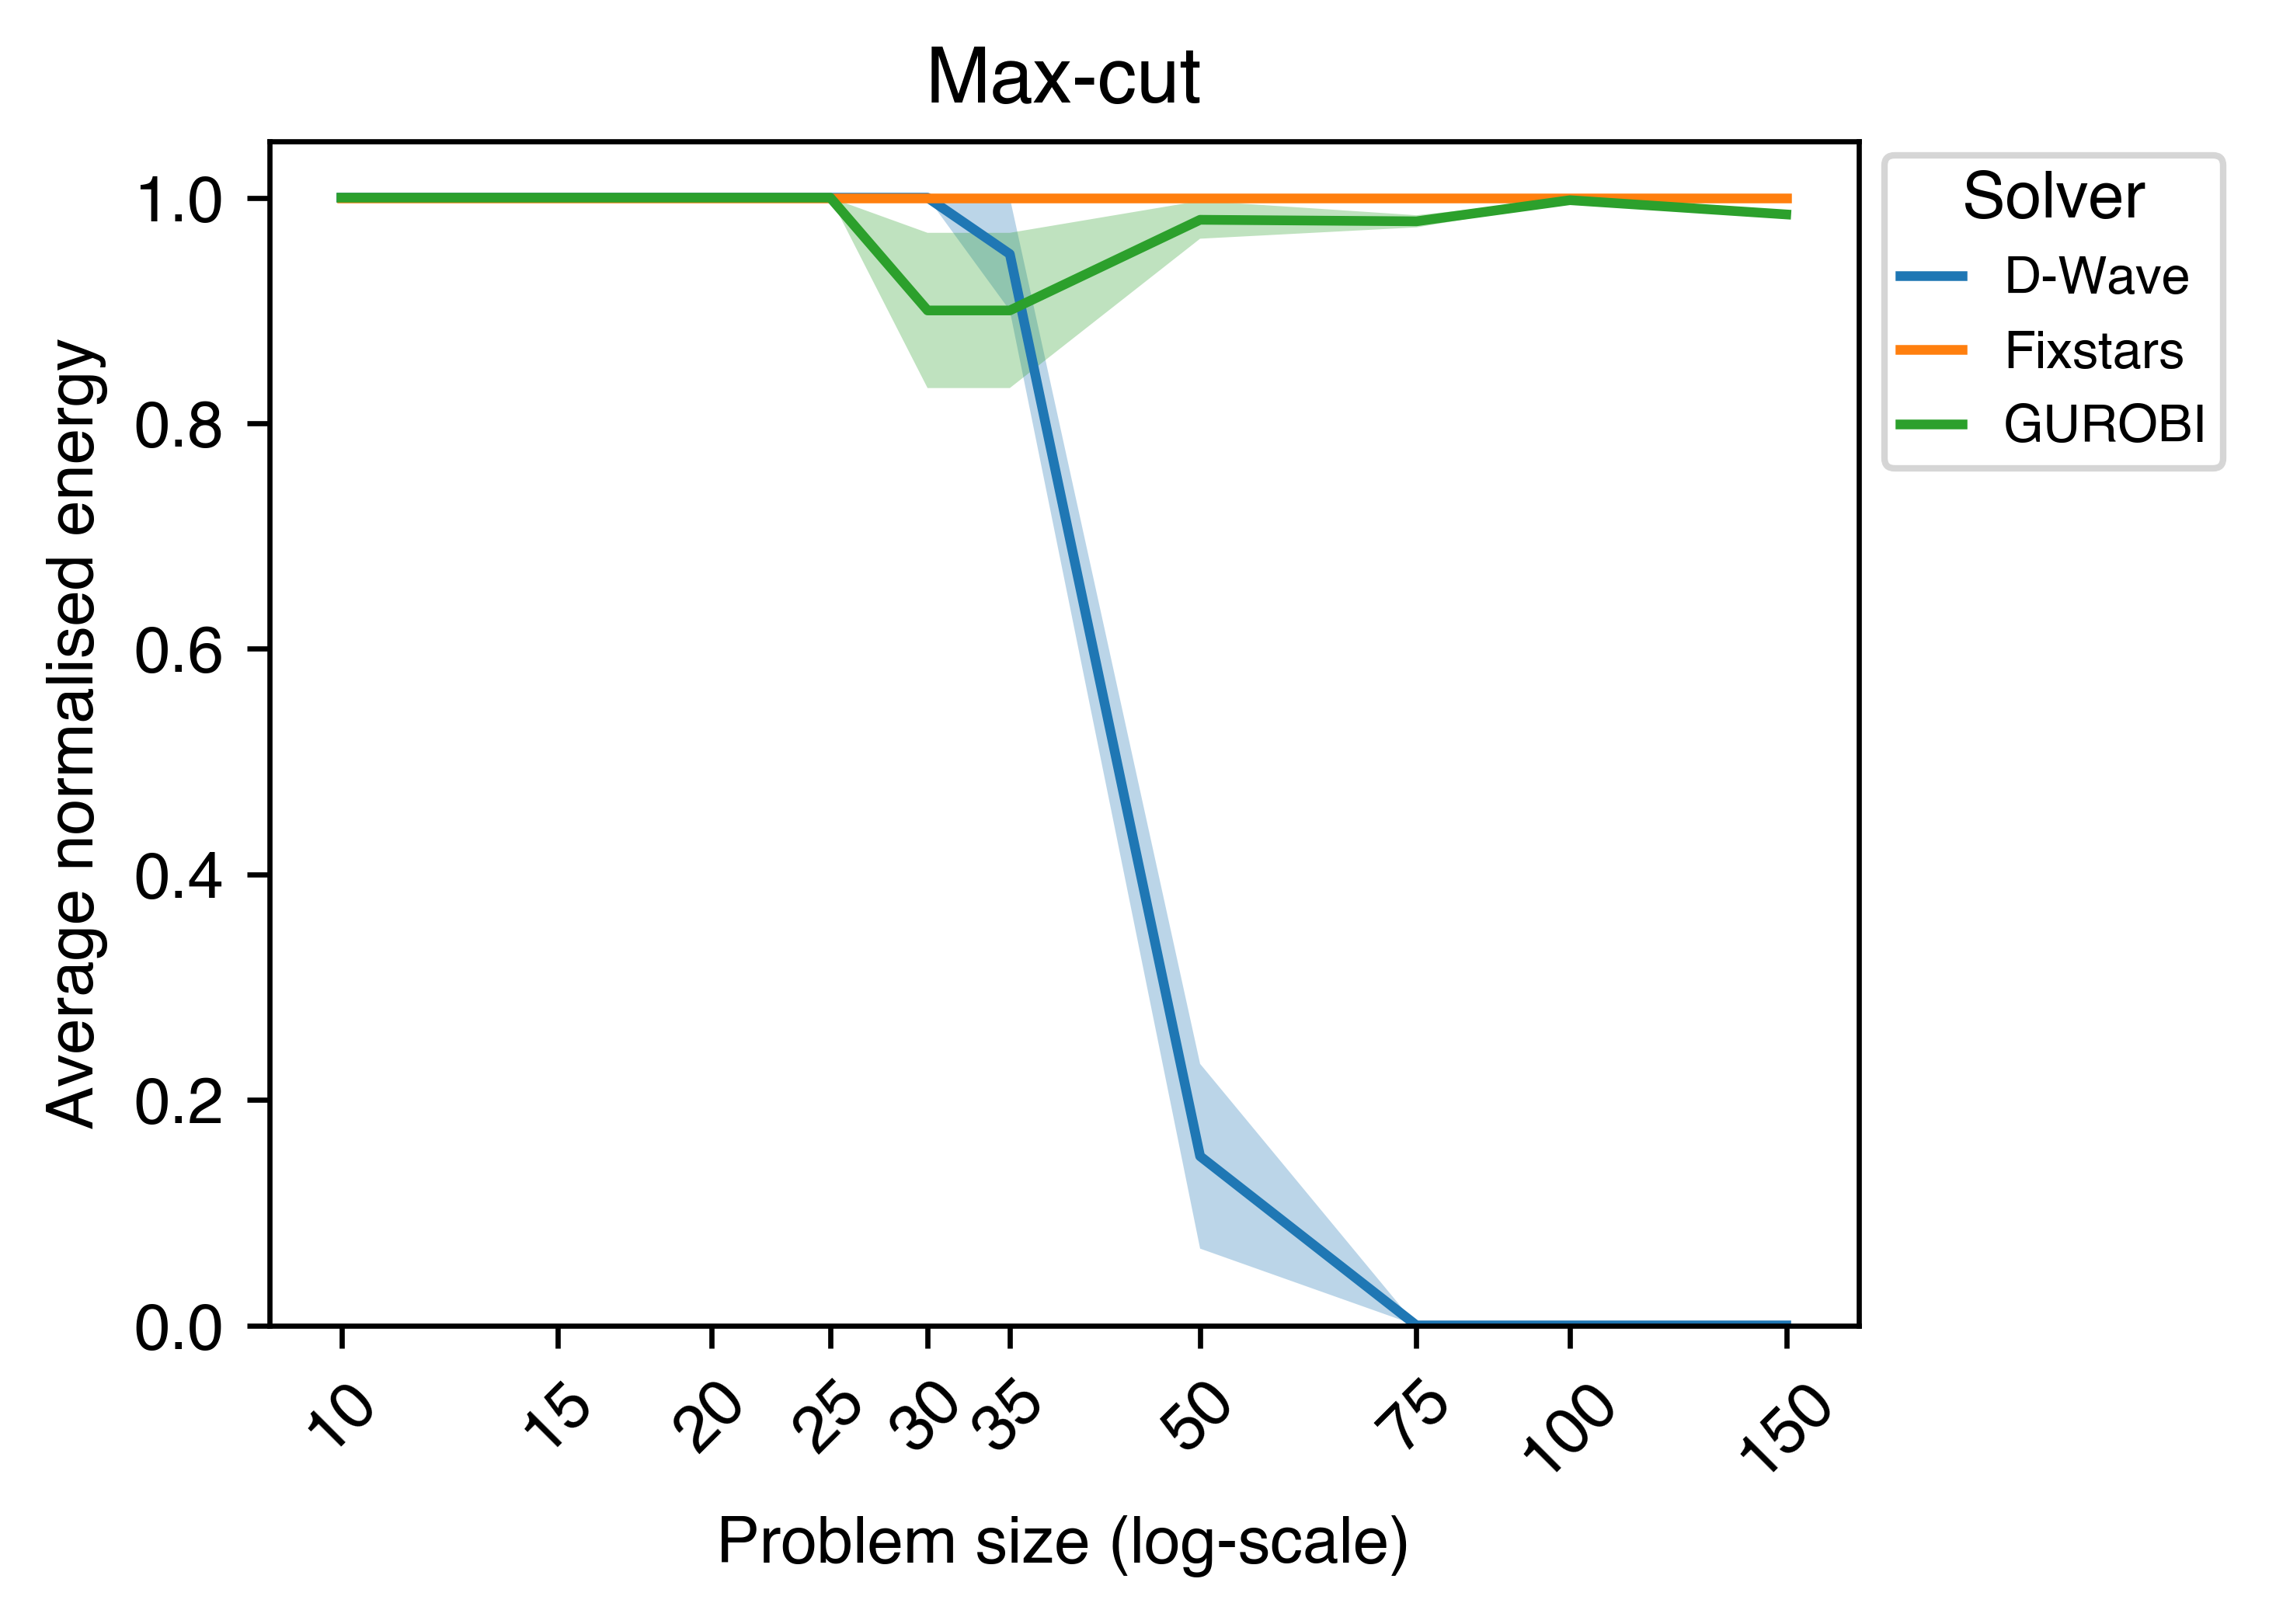
\includegraphics[width=0.5\textwidth]{images/maxcut_timing_size.png}}
    \\    
    \subfloat[SK model]{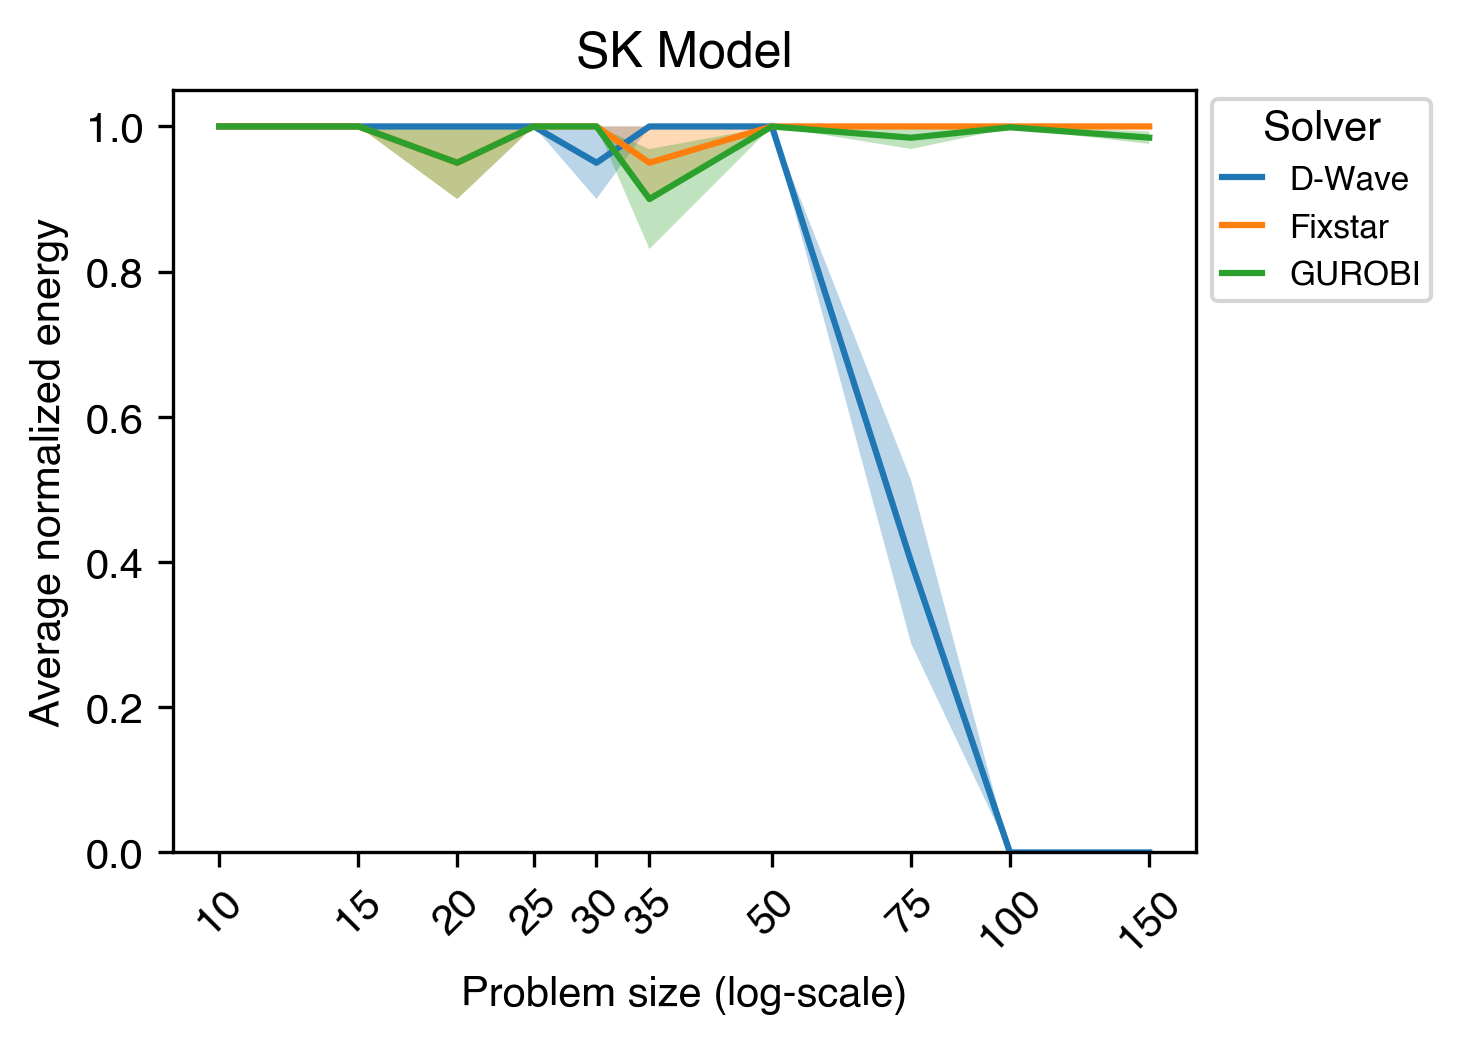
\includegraphics[width=0.5\textwidth]{images/skmodel_timing_size.png}}
    \caption{Average normalised energy of D-Wave solver against the GUROBI and Fixstar solvers by problem type and size}
    \label{all-time-size}
\end{figure}

\section{Additional Solver Information}
Additional D-Wave and QAOA solver information was recorded during the benchmarking experiments. This information helps quantify the difficulty of a QUBO problem for a particular solver and could be used to classify different types of QUBO problems.
\subsection{D-Wave}
For the D-Wave solver, we recorded the average number of embedded qubits shown in \autoref{table:numberofembedded}, generated during the minor embedding phase when a single qubit is split into a chain. The number of embedded qubits increases at different rates for different problem types and could be a metric for the difficulty of the annealing problem. The number of embedded qubits also limits the problems the D-Wave solver can handle since the QPU only has $\sim 5000$ qubits.
\begin{table}[!htb]
    \centering
    \resizebox{\textwidth}{!}{%
    \tabcolsep=0.1cm
    \begin{tabular}{lrrrrrrrrrrrrr} \toprule
        $n$ & 10 & 15 & 20 & 25 & 30 & 35 & 50 & 75 & 100 & 150 & 200 & 250 & 300 \\ \midrule
        NAE3SAT & 15.15 & 27.90 & 42.20 & 58.85 & 80.90 & 102.25 & 184.05 & 379.65 & 622.15 & 1381.00 & 2322.65 & 3756.20 & 4493.60 \\
        Max-cut & 12.70 & 25.95 & 45.45 & 69.90 & 102.60 & 142.50 & 304.05 & 706.05 & 1290.00 & 3087.95 & - & - & - \\
        SK model & 17.05 & 35.80 & 54.50 & 87.65 & 121.15 & 169.80 & 331.60 & 739.45 & 1338.65 & 2995.25 & - & - & - \\ \bottomrule
    \end{tabular}}
    \caption{Average number of embedded qubits for the D-wave solver by problem type and size}
    \label{table:numberofembedded}
\end{table}
\subsection{QAOA}
For the QAOA solver, we recorded the number of quantum gates and the circuit depth, shown in \autoref{table:gates} and \autoref{table:depth}, respectively, which can help quantify the complexity of the quantum circuit used and the requirements needed for a quantum computer to run the QAOA solver.
\begin{table}[!htb]
    \centering
    \small
    \begin{tabular}{lrrrrr} \toprule
        $n$ & 10 & 15 & 20 & 25 & 30\\ \midrule
        NAE3SAT & 77.75 & 127.80 & 181.50 & 235.20 & 292.30 \\
        Max-cut & 75.00 & 131.00 & 200.00 & 281.00 & 375.00 \\
        SK model & 95.00 & 180.00 & 290.00 & 425.00 & 585.00\\ \bottomrule
    \end{tabular}
    \caption{Average number of quantum gates in the quantum circuit used by the QAOA solver by problem type and size}
    \label{table:gates}
\end{table}

\begin{table}[!htb]
    \centering
    \begin{tabular}{lrrrrr} \toprule
        $n$ & 10 & 15 & 20 & 25 & 30\\ \midrule
        NAE3SAT & 18.65 & 25.30 & 30.70 & 35.15 & 40.00 \\
        Max-cut & 19.00 & 28.05 & 36.50 & 45.60 & 55.05 \\
        SK model & 22.00 & 32.00 & 42.00 & 52.00 & 62.00\\ \bottomrule
    \end{tabular}
    \caption{Average depth of the quantum circuit used by the QAOA solver by problem type and size}
    \label{table:depth}
\end{table}

\section{Conclusion}
\autoref{results:allnormalizedenergy} and \autoref{results:allsuccess} show the average normalised energy and success probability for different solvers for each dataset and also the average value across all datasets. Among the three quantum-inspired solvers, the NNQS solver has the best normalised energy for the NAE3SAT and max-cut dataset, while the D-Wave solver has the best normalised energy for the SK model performance. The NNQS solver also has the highest normalised energy when averaged across the three datasets. 

The QAOA solver has the highest success probability for the NAE3SAT dataset, however, it can only handle problems with up to $30$ variables. The D-Wave solver has the best success probability for the max-cut and SK model datasets while doing better than the NNQS solver for the NAE3SAT dataset. When averaged across the three datasets, the D-Wave solver has the highest success probability.

The NNQS solver tends to do better in normalised energy since it minimises the energy expectation value and consistently finds low-energy solutions. Conversely, the D-Wave solver is better at finding the best solution. The two solvers have different strengths and may be suited for different optimisation tasks.

Across all datasets and metrics, the Fixstar solver has the best performance, consistently returning the best solutions for almost all problem types and sizes. The GUROBI solver also does well, except for large problems ($n\geq 250$). When the runtimes are matched, the D-Wave solver can outperform the GUROBI solver for specific problem sizes but still underperforms the Fixstar solver. 

\begin{table}[!htb]
    \centering
    \begin{tabular}{cccccc} \toprule
        ~ & D-Wave & NNQS & QAOA & GUROBI & Fixstar \\ \midrule
        NAE3SAT & 0.617 & \textbf{0.755} & 0.640 & 0.983 & 1.00 \\
        Max-cut & 0.610 & \textbf{0.753} & 0.190 & 0.991 & 1.00 \\
        SK model & \textbf{0.761} & 0.664 & 0.230 & 0.990 & 1.00 \\ \midrule
        Average & 0.663 & \textbf{0.724} & 0.353 & 0.988 & 1.00 \\ \bottomrule
    \end{tabular}
    \caption{Average normalised energy for different solvers}
    \label{results:allnormalizedenergy}
\end{table}

\begin{table}[!htb]
    \centering
    \begin{tabular}{cccccc} \toprule
        ~ & D-Wave & NNQS & QAOA & GUROBI & Fixstar \\ \midrule
        NAE3SAT & 0.615 & 0.538 & \textbf{0.640} & 0.858 & 1.00 \\
        Max-cut & \textbf{0.610} & 0.585 & 0.190 & 0.931 & 1.00 \\
        SK model & \textbf{0.740} & 0.538 & 0.230 & 0.954 & 1.00 \\ \midrule
        Average & \textbf{0.655} & 0.554 & 0.353 & 0.914 & 1.00 \\ \bottomrule
    \end{tabular}
\caption{Success probability for different solvers}
\label{results:allsuccess}
\end{table}

